
\section{Kolkkien ja seikkalijoiden päiväretki 13.4.}

% \vspace*{-0.16cm}
\begin{center}
	\noindent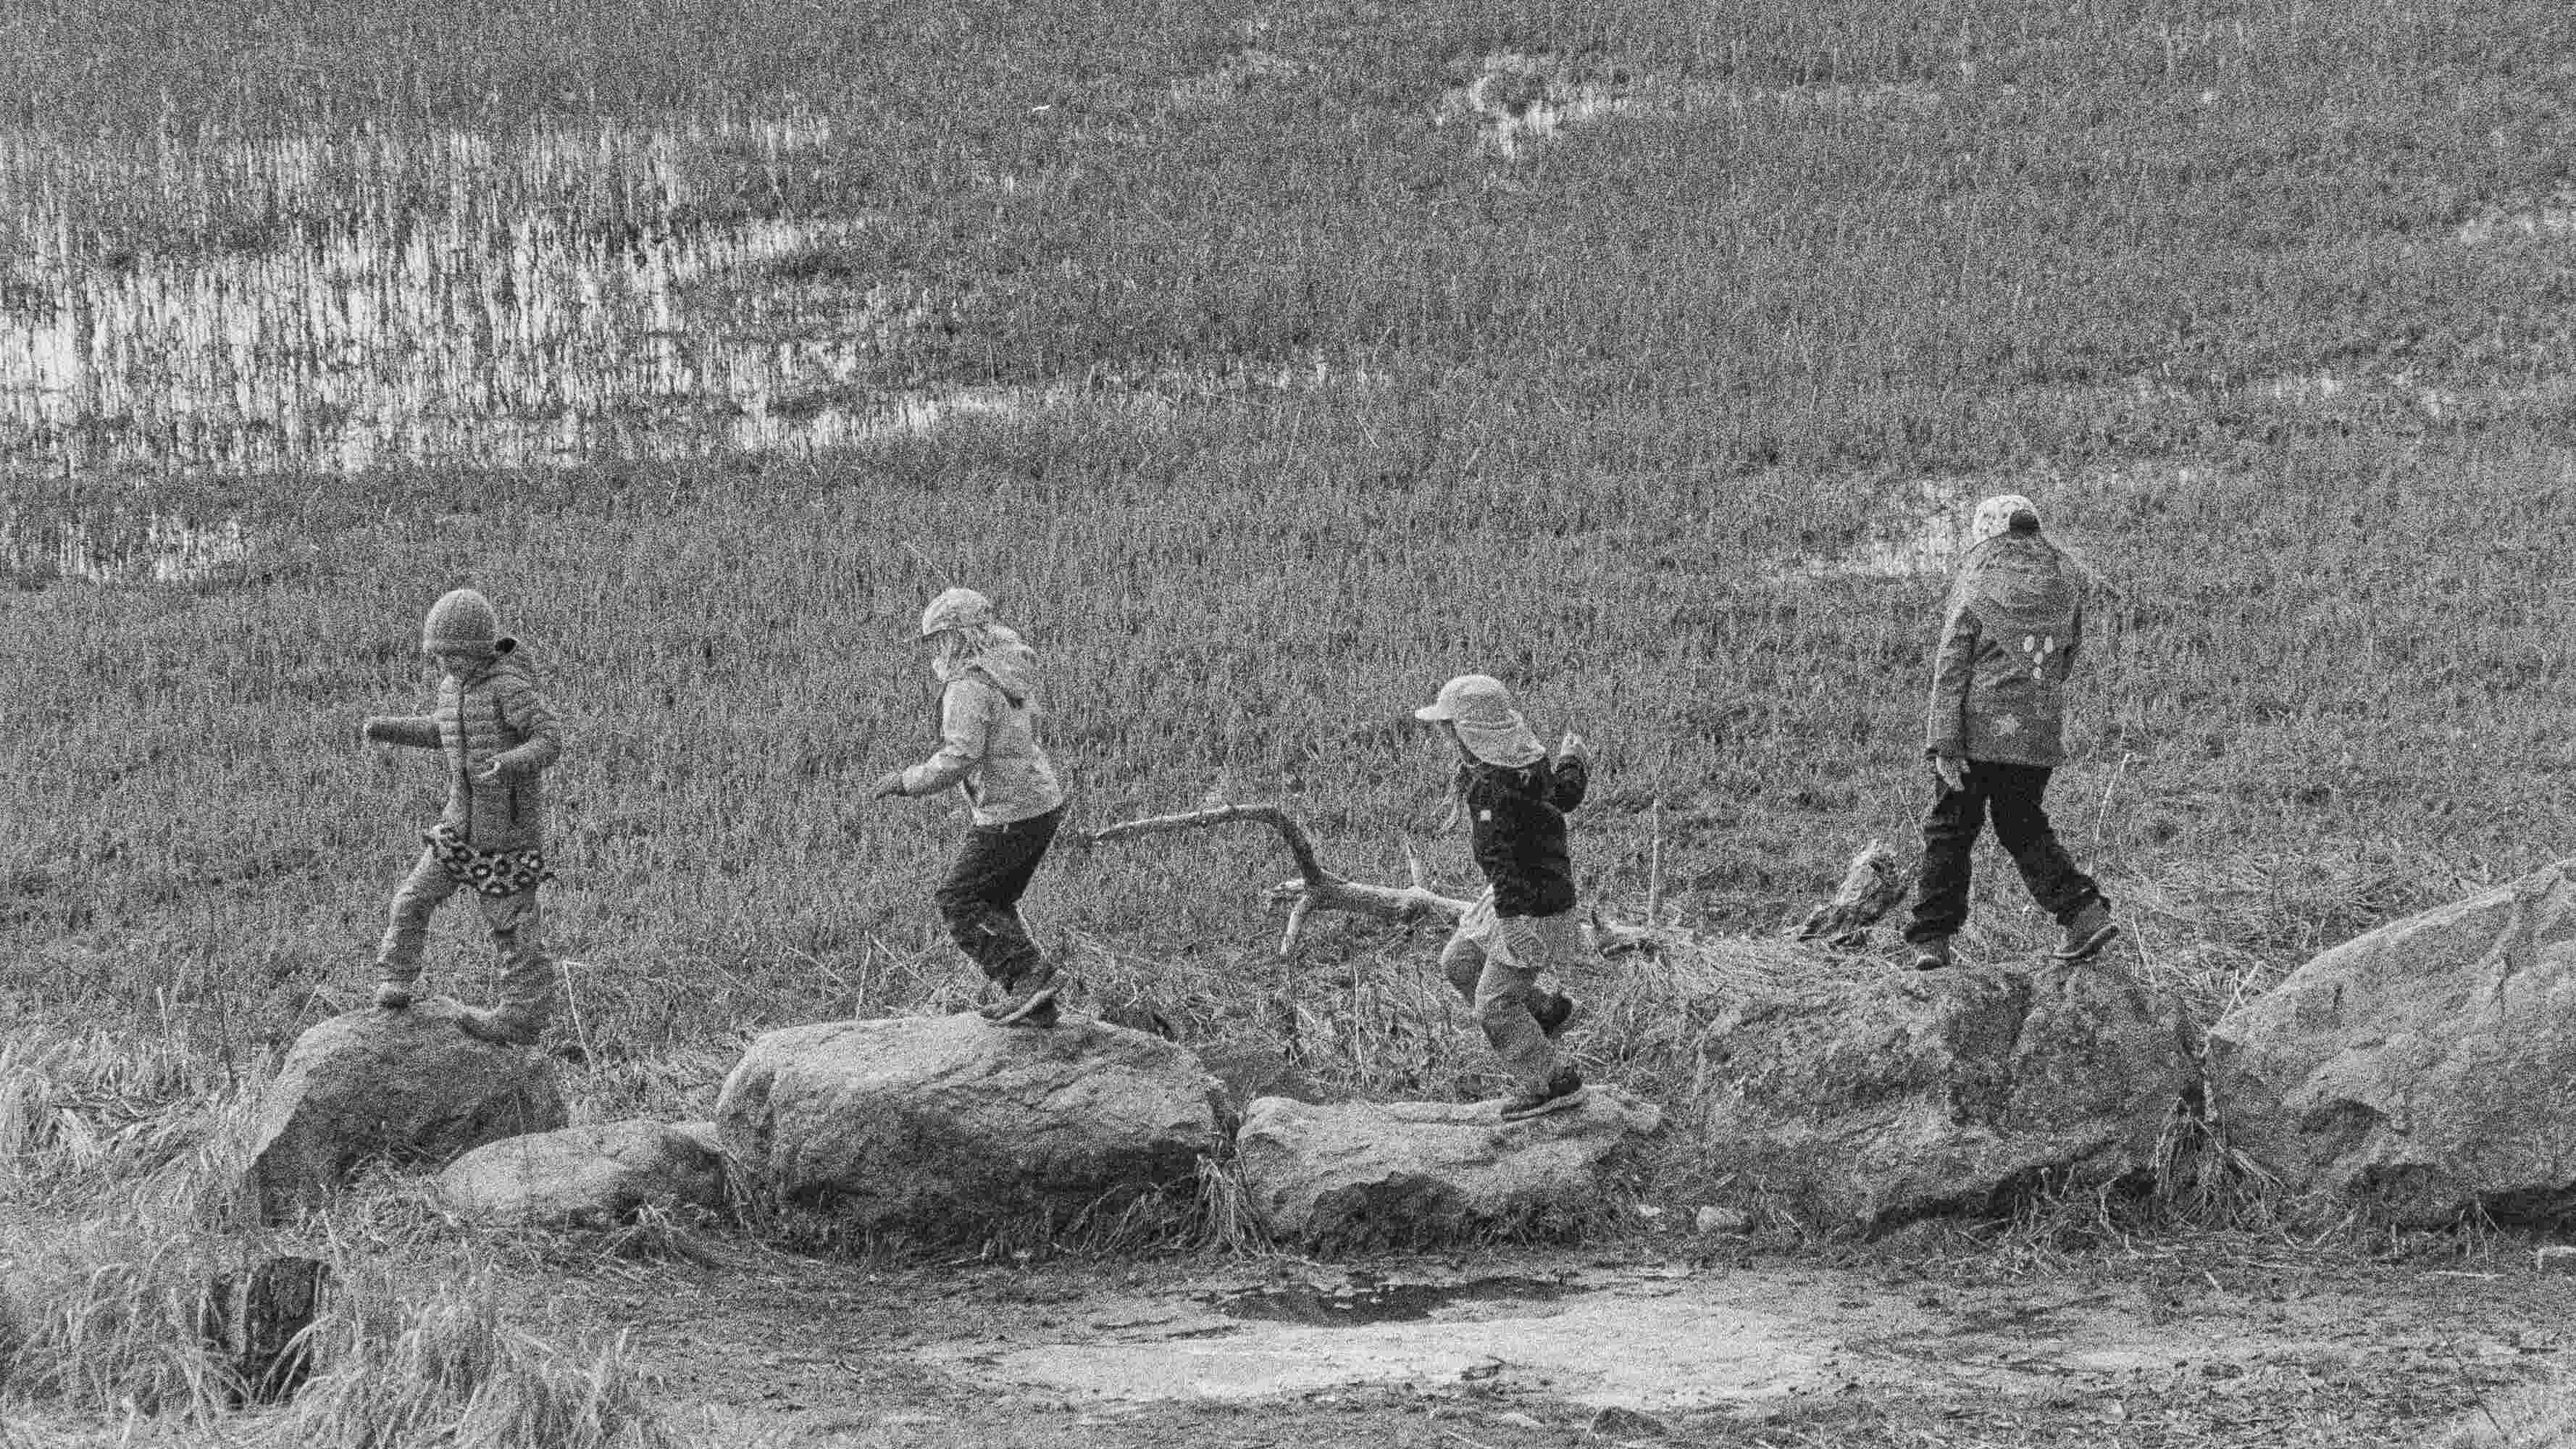
\includegraphics[width=0.8\linewidth]{assets/kolkkienpäiväretkibw3}
\end{center}
\vspace*{-0.16cm}

\begin{multicols}{2}

	\noindent Lippukunnan kolkat ja seikkailijat tekivät yhteisen päiväretken
	huhtikuisena lauantaina. Retkue kokoontui ohjeistetusti Kivikossa
	Järkälekujan bussipysäkillä, jonne Alisa, Annina, Elna, Janja, Janne,
	Johannes, Kuisma, Lillian, Nella, Sade, Tanguy ja Veera (harmillisesti
	ainoa retkelle ilmoittautunut seikkailija oli sairastunut) saapuivat
	kaikki niin hyvissä ajoin, että retkue pääsi suunniteltua aikaisemman
	bussin kyytiin – mitä nyt muutamaa kolkkaa piti kiiruhtaa lopettamaan
	terveysaseman kallioilla kiipeileminen.

	Bussista jäätiin Latokartanon pysäkillä, josta käveltiin reippaasti
	entisen puutarhan, nykyisen olutpanimon läheiselle parkkipaikalle.
	Parkkipaikalle olivatkin juuri parahiksi saapuneet myös Ilona, Jella,
	Leo ja Nonna, joiden autosta otettiin kantoon vesi ja tiskivadit.
	\mbox{Retki Viikinrannan} kevätluontoon voi \mbox{alkaa!}

	Pari sataa metriä myöhemmin jo pysähdyttiin entisen maatalousmuseon
	edessä ihmettelemään puuhun kiinnitettyä ohjeistusta:
	Pistelaskentapaikka Jyväskylän yliopistossa kehitetylle Muuttolintujen
	Kevät -mobiilisovellukselle, jonka "avulla sinulla on mahdollisuus
	tallentaa linnunlaulua ja tehdä lintuhavaintoja hyödyntäen modernia
	tekoälyä". Pikemmittä puheitta retkenjohtaja Annina otti puhelimen
	esiin ja aloitti viiden minuutin mittauksen, jonka aikana tuli olla
	aivan hiljaa. Vaikka viisi minuuttia tuntui ehkä joistakuista
	ikuisuudelta, meni aika kuitenkin nopeasti ilman ylimääräistä
	metelöintiä luonnon ääniä kuunnellen.

	\columnbreak

	(Toim. huom. havaintoaineisto on avointa ja löytyy valmiiksi kartalta
	esimerkiksi täältä:
	\href{https://yle.fi/aihe/a/20-10004726}{https://yle.fi/aihe/a/20-10004726}.
	Retken laskentapaikalle on merkitty 13.4. kalalokki, kuovi,
	sepelkyyhky, talitiainen ja varis – osa mahdollisesti meidän tekemän
	mittauksen ansiosta! Sunnuntaihin 14.4. mennessä sovelluksella oli
	kerätty yli kolme miljoonaa äänitystä Helsingissä ja Jyväskylässä
	tutkijoiden käyttöön.)

	Hiljaisuusharjoituksen jälkeen jatkettiin kohti Keinumäen lintutornia,
	jonka läheisyydessä oli määrä laittaa lounasta – kolkat kun suorittivat
	keväällä retkikokki-jälkeä. Viikin puupuiston tietämillä Tanguy
	ohjeisti retkeläisille lintubingon, jossa merkinnän ruudukkoon sai
	tehdä esimerkiksi linnun keltaisesta nokasta, uivasta linnusta ja
	laulavasta talitiaisesta. Ensimmäinen bingo saatiin jo ennen Keinumäkeä
	ja palkittiin asianmukaisesti rusinoilla.

	\begin{Figure}
		\noindent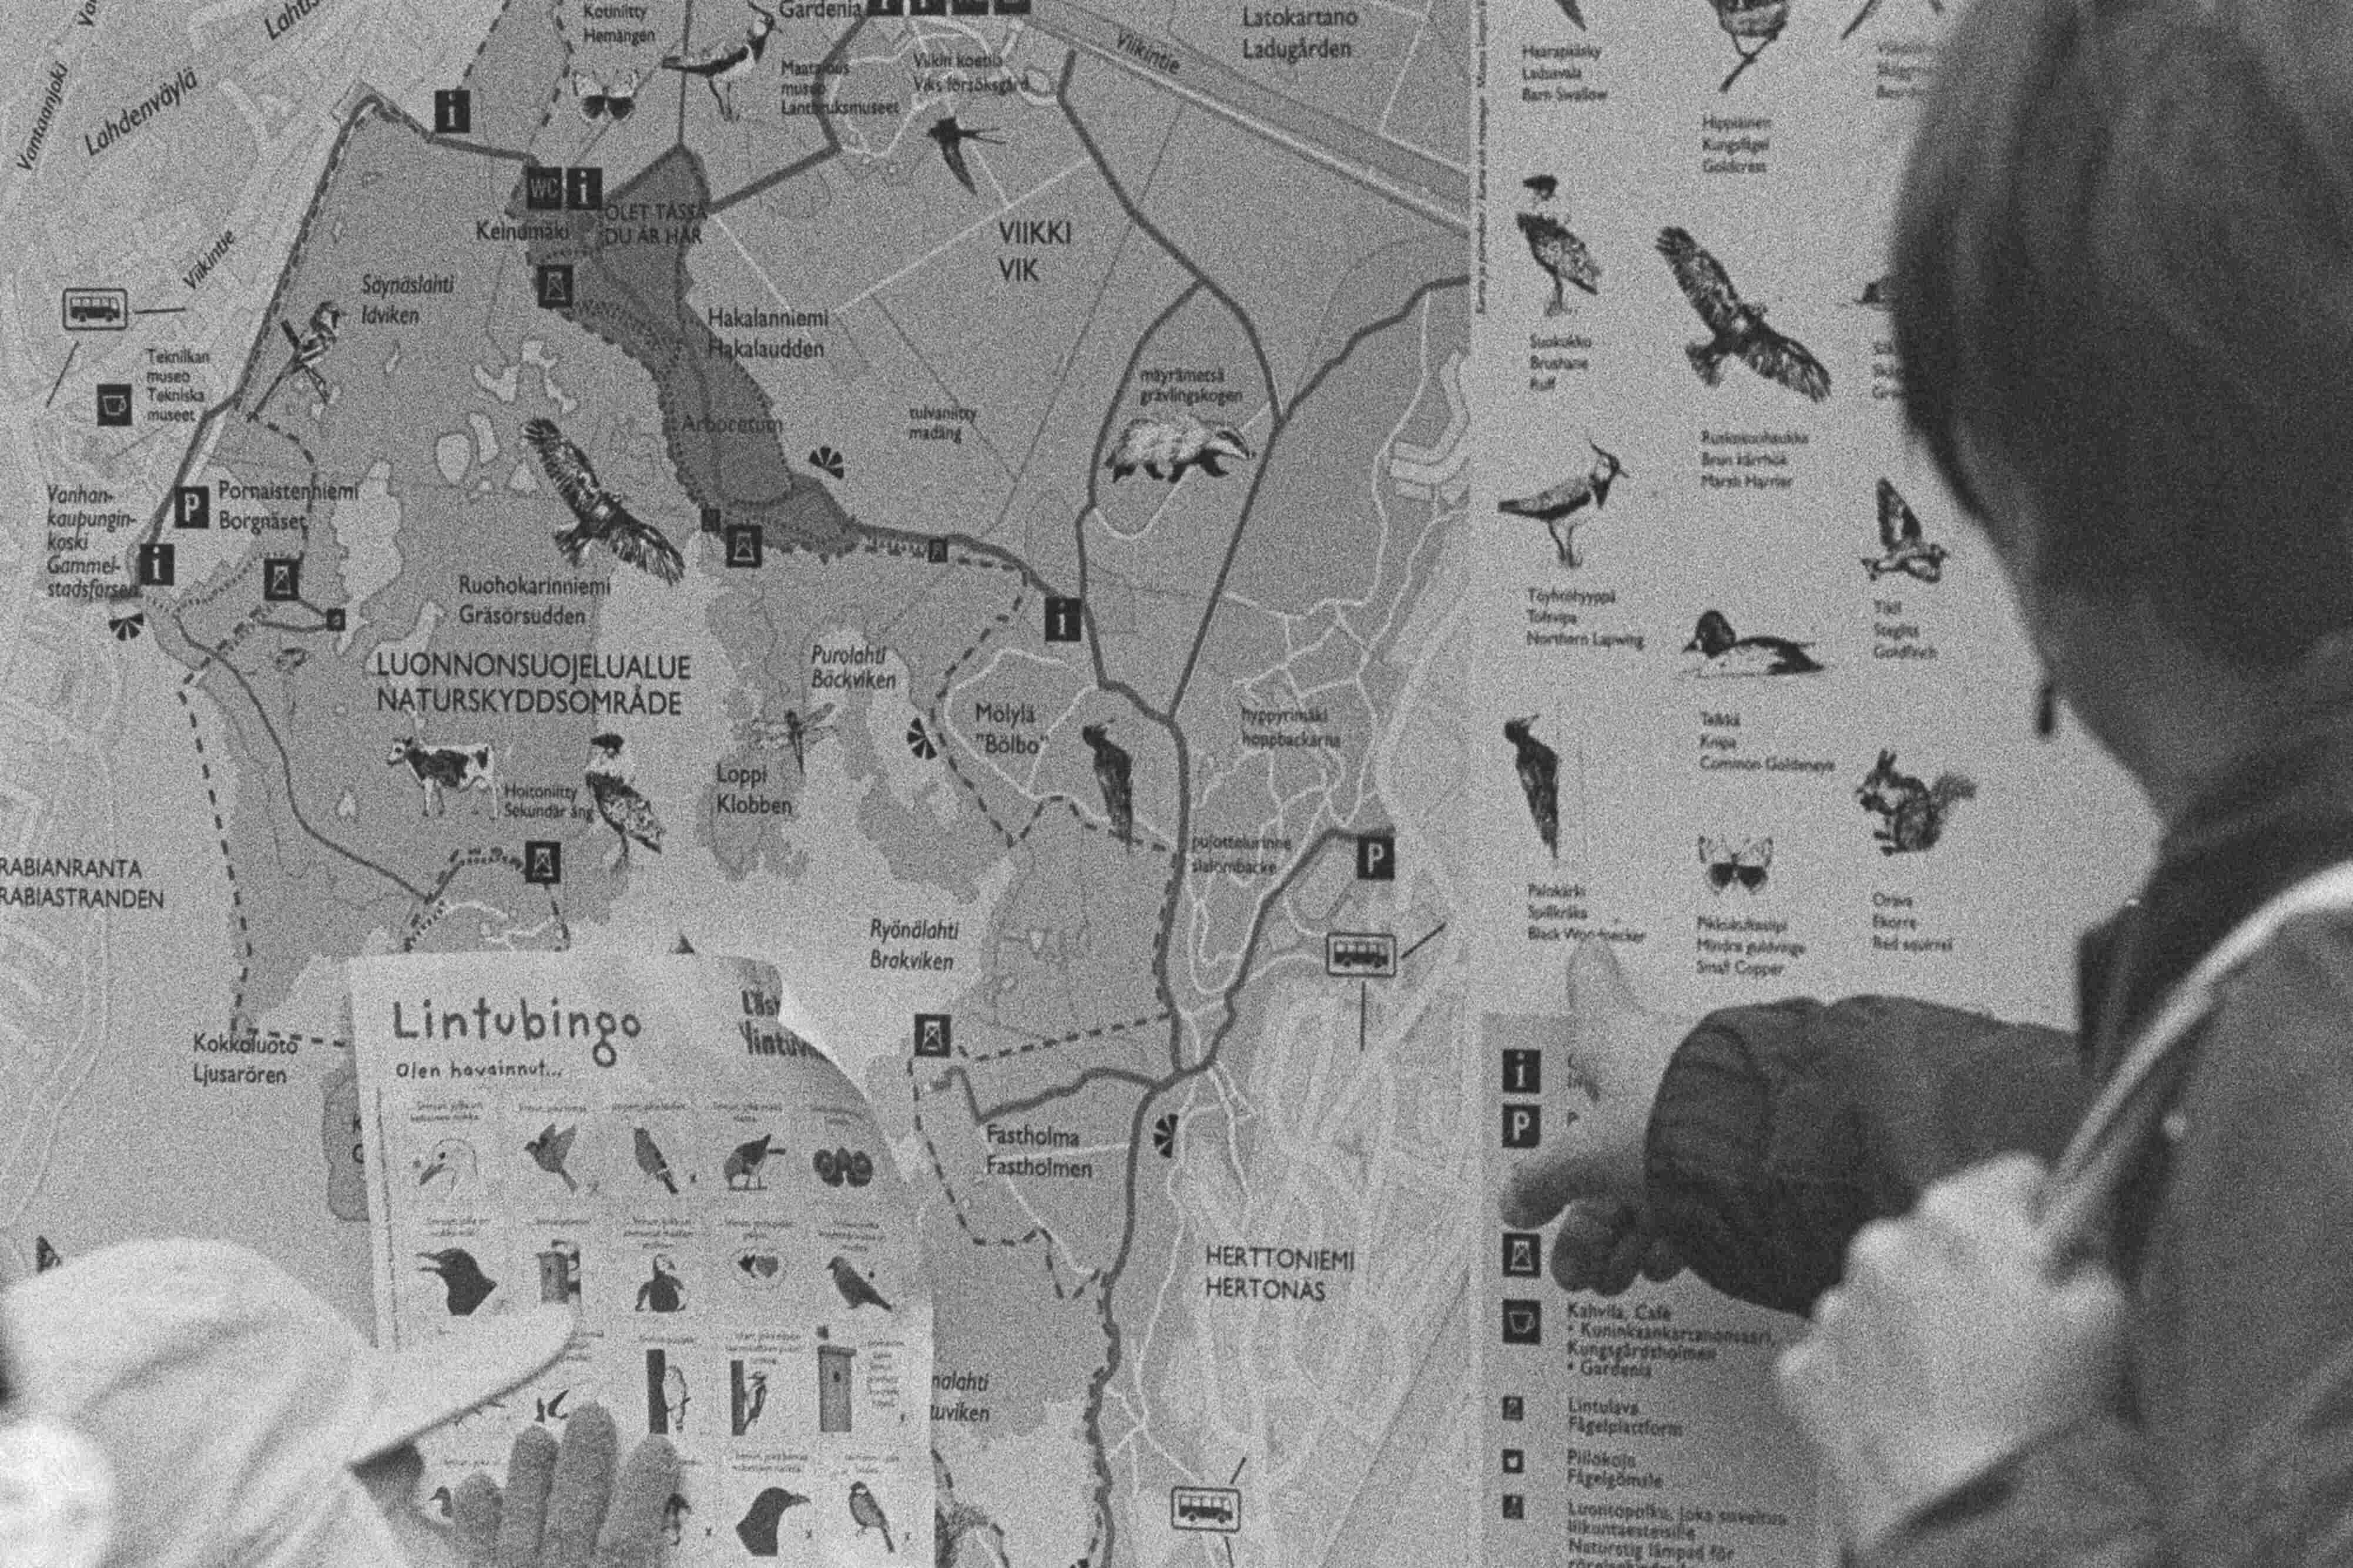
\includegraphics[width=\linewidth]{assets/kolkkienpäiväretkibw1}
	\end{Figure}

	Lyhyt pysähdys opastauluilla ja oltiin jo lintutornilla. Trangiat
	kaivettiin esiin ja aloitettiin ruoanvalmistus; kolkat olivat
	suunnitelleet retkelle kahden ruokalajin aterian valmiiksi kevään
	kokouksissaan. Pääruoaksi oli vegaanista nakkikeittoa ja jälkiruoaksi
	kaura-omenapaistosta vaniljakastikkeella. Keitto valmistui varsin
	jouhevasti, vaikka jotkut retkeläiset olivatkin innokkaammin
	leikkimässä kuin leikkaamassa nakkeja ja omenoita. Veden kiehumista
	odotellessa halukkaat pääsivät myös kiipeämään lintutorniin seuraamaan
	lintuja Vanhankaupunginlahdella. Kevätmuutto oli vasta aluillaan, minkä
	vuoksi lintuja ei havaittu aivan yhtä paljon kuin BirdLife Suomen
	Tornien taisto -kilpailussa vuonna 2023 (102 lintulajia/8 tuntia).

	% \vspace*{-0.32cm}
	\begin{center}
		\noindent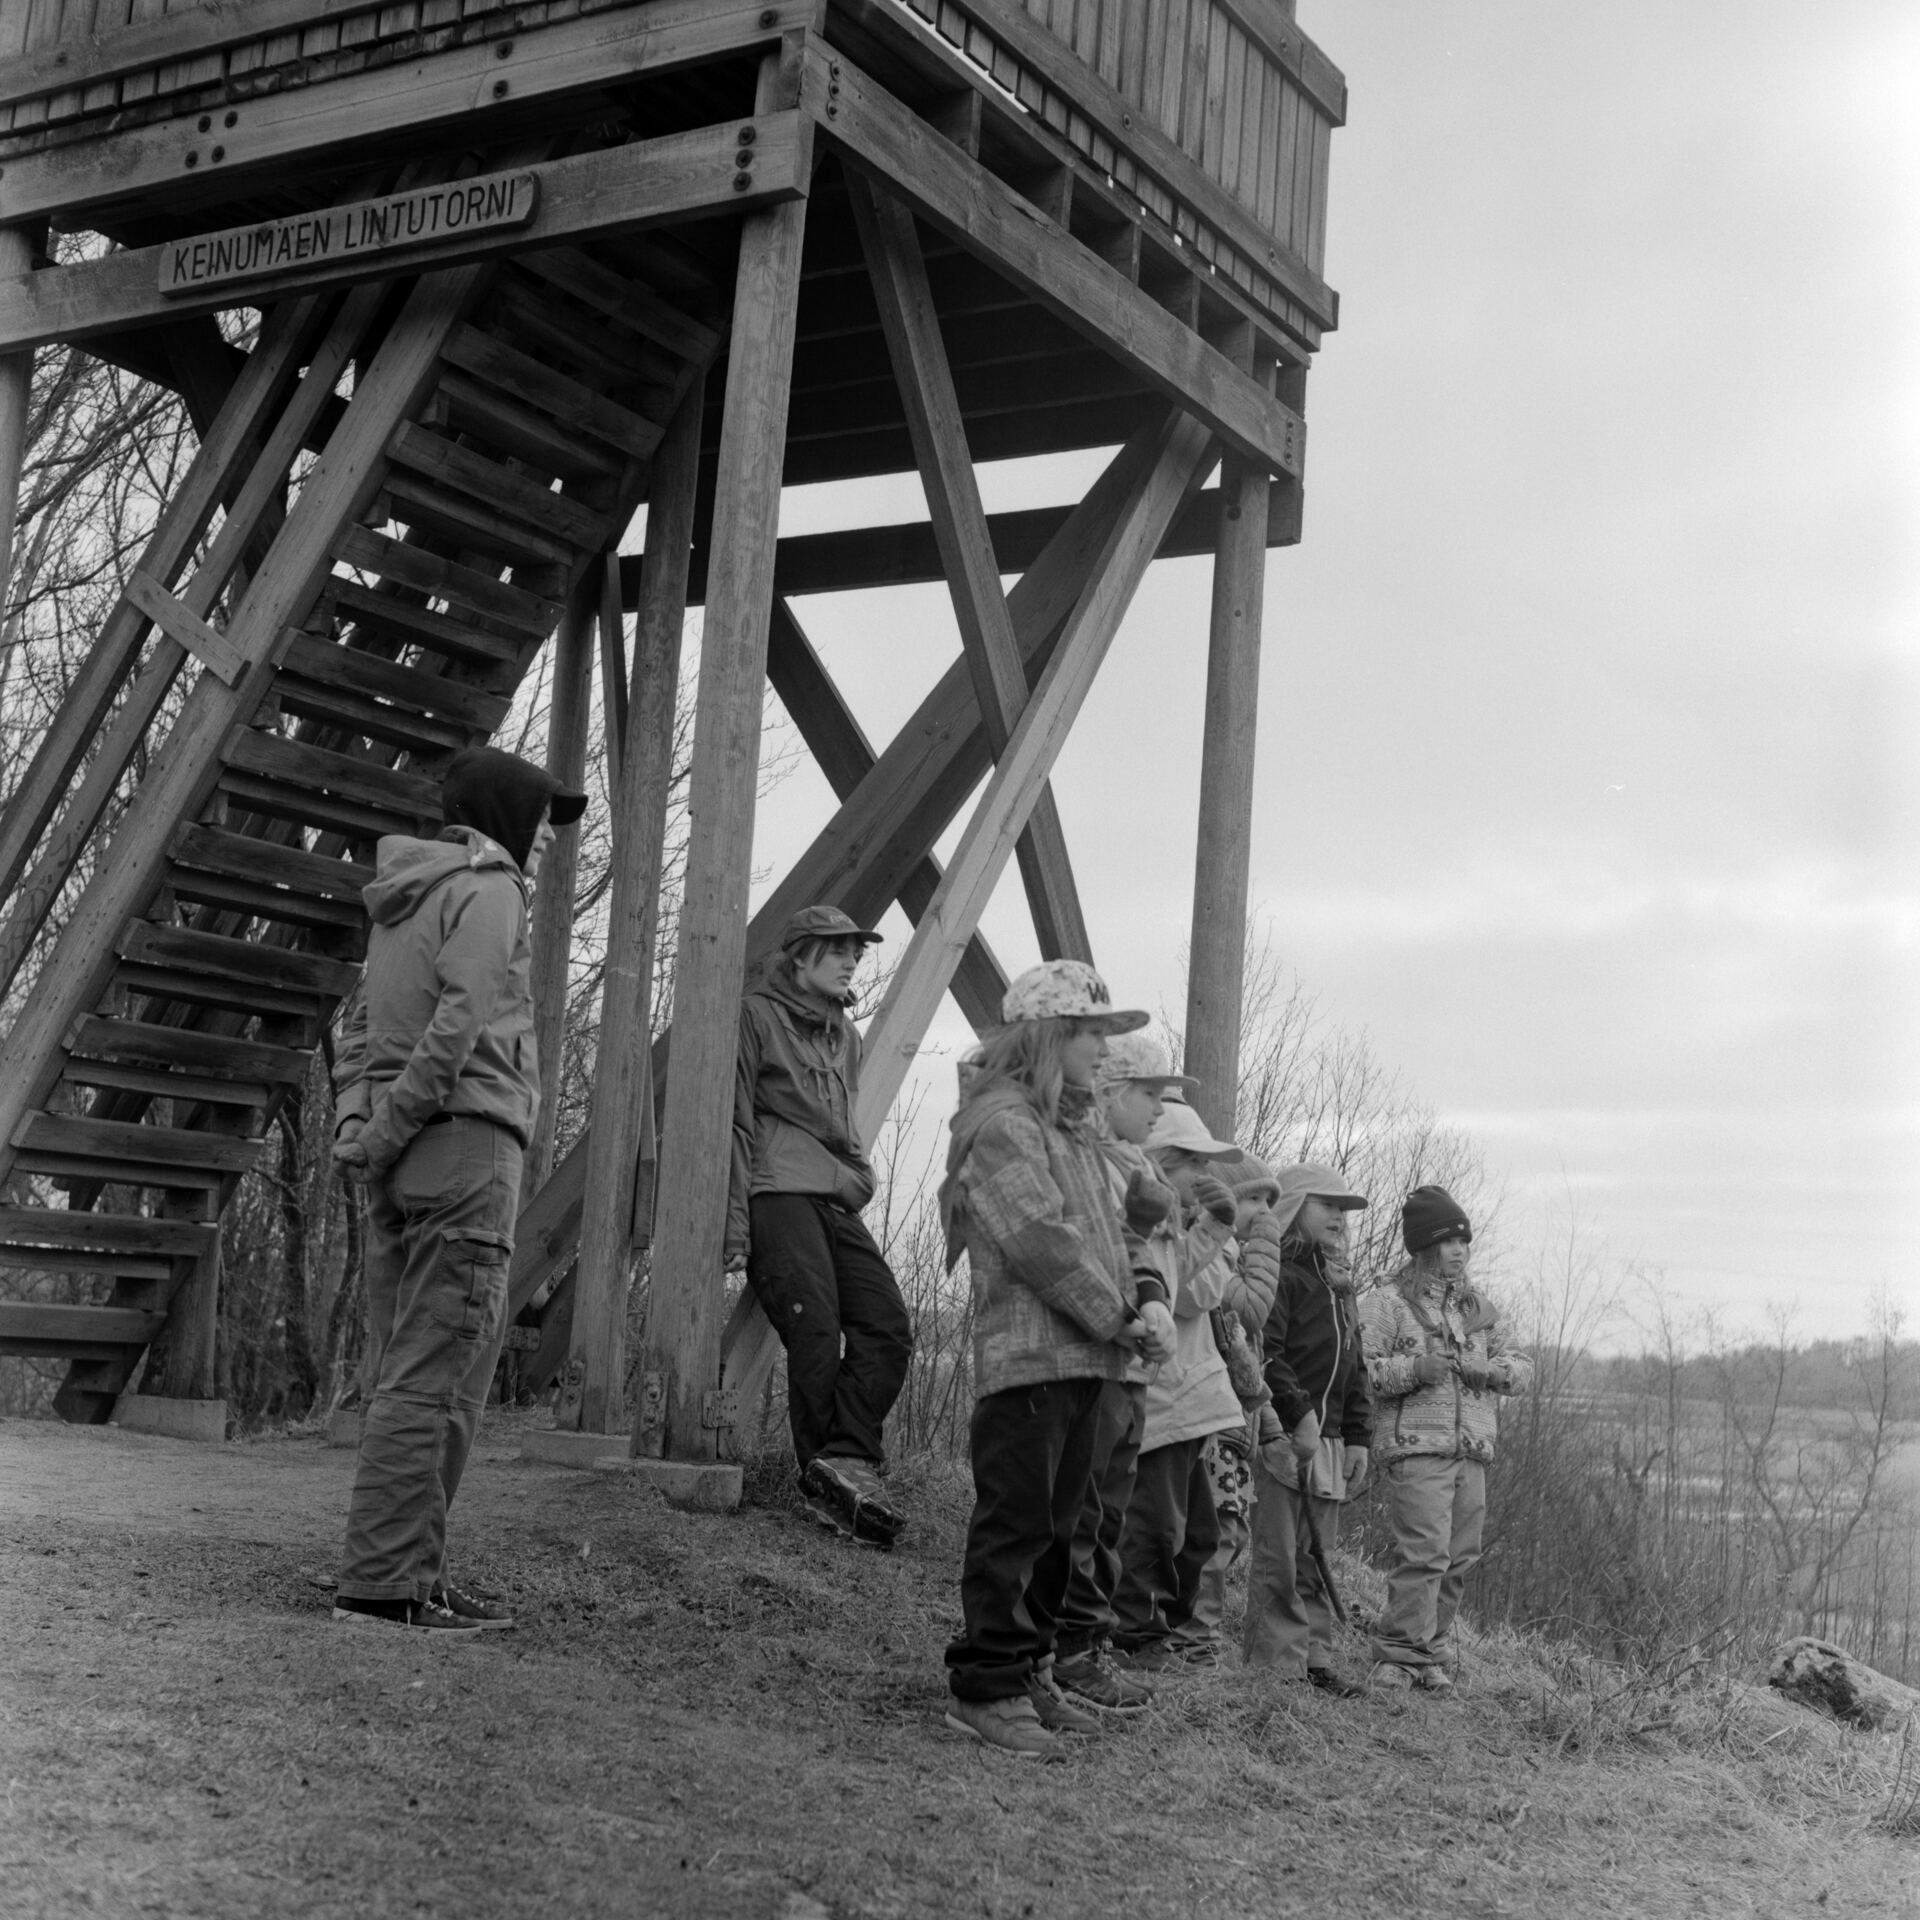
\includegraphics[width=0.8\linewidth]{assets/kolkkienpäiväretkibw15}
	\end{center}

	Keittojuuresten kiehuessa nälkä alkoi jo kurnimaan ja viimein saatiin
	oikein herkullista keittoa – lämmikkeeksi sulan meren yli puhaltaneen
	tuulen jäähdyttämille retkeilijöille. Onneksi jälkiruoka valmistui
	nopeammin. Paistosta oltiin koeajettu kolkkien kokouksessa jo
	aikaisemmin keväällä ja suurta makunautintoa kannatti odottaa. Retken
	alkupään viiden minuutin mittainen hiljaisuus oli tässä vaiheessa
	muuttunut jo hataraksi muistikuvaksi, kun retkeläisten äänenkäyttö
	hipoi häiritsevän voimakasta meteliä. 

	% \columnbreak

	% \vspace*{-0.64cm}
	\begin{center}
		\noindent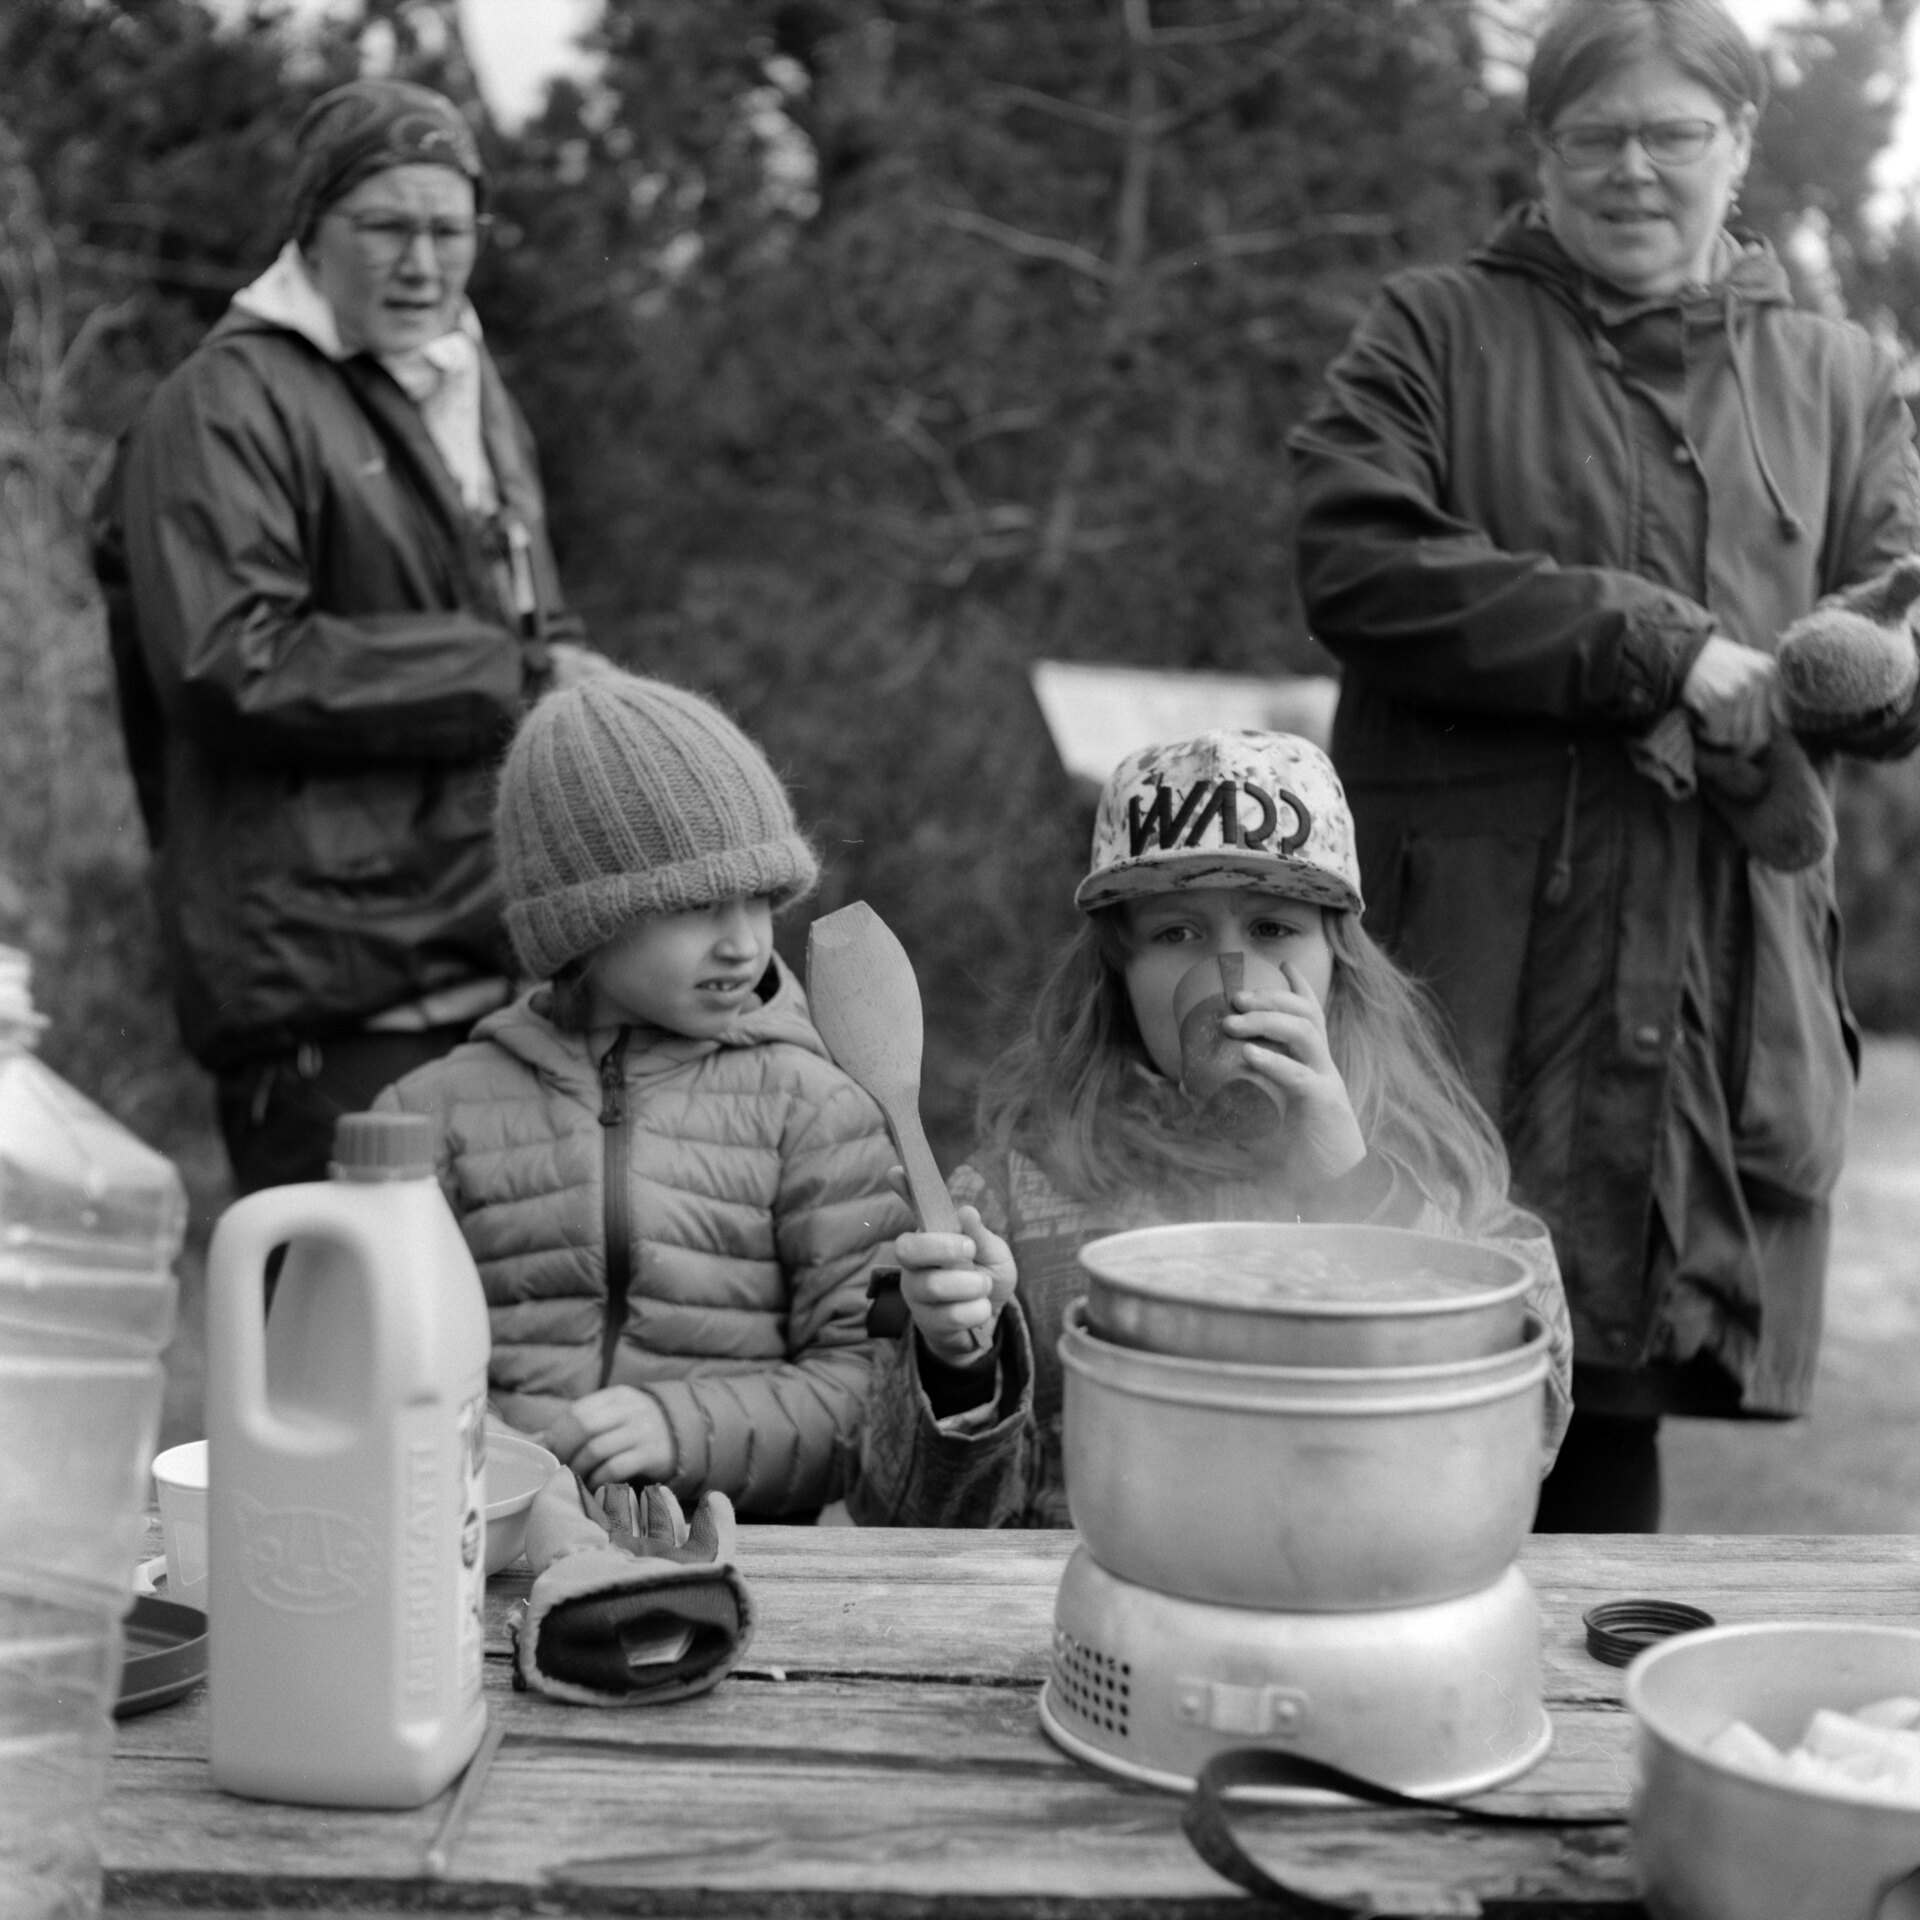
\includegraphics[width=0.8\linewidth]{assets/kolkkienpäiväretkibw14}
	\end{center}

	Retkikokki-jälkeen sisältyi luonnollisesti myös tiskaus. Kukin
	retkeläinen tiskasi omat astiansa ja trangiat, minkä jälkeen tehtiin
	ilmaisuharjoituksia Leon johdolla. Partiolaiset eivät jätä jälkeensä
	jälkiä, mikä toteutui retkellä lähes erinomaisesti. Ainoastaan yksi
	trangian polttimon kierrekorkki jäi jälkeen etsinnöistä huolimatta.

	% \columnbreak

	Johannes lähti isänsä kanssa valmistautumaan illan teatterinäytökseen
	ja muut siirtyivät retken rastitehtäviin. Rasteilla retkeläiset
	pääsivät oppimaan uusia kasvien ja jäkälien nimiä
	Jumbobonus-hippaleikissä, ilmaisemaan luovuuttaan ja kekseliäisyyttään
	tekemällä miniatyyri-installaation, verestämään muistiaan lintulajien
	muistipelissä sekä löytämään sisäisen valokuvaajansa ottamalla hauskoja
	valokuvia – joita voit nähdä seuravalla sivulla!

	% \vspace*{0.16cm}

	\vspace*{0.16cm}
	\begin{center}
		\noindent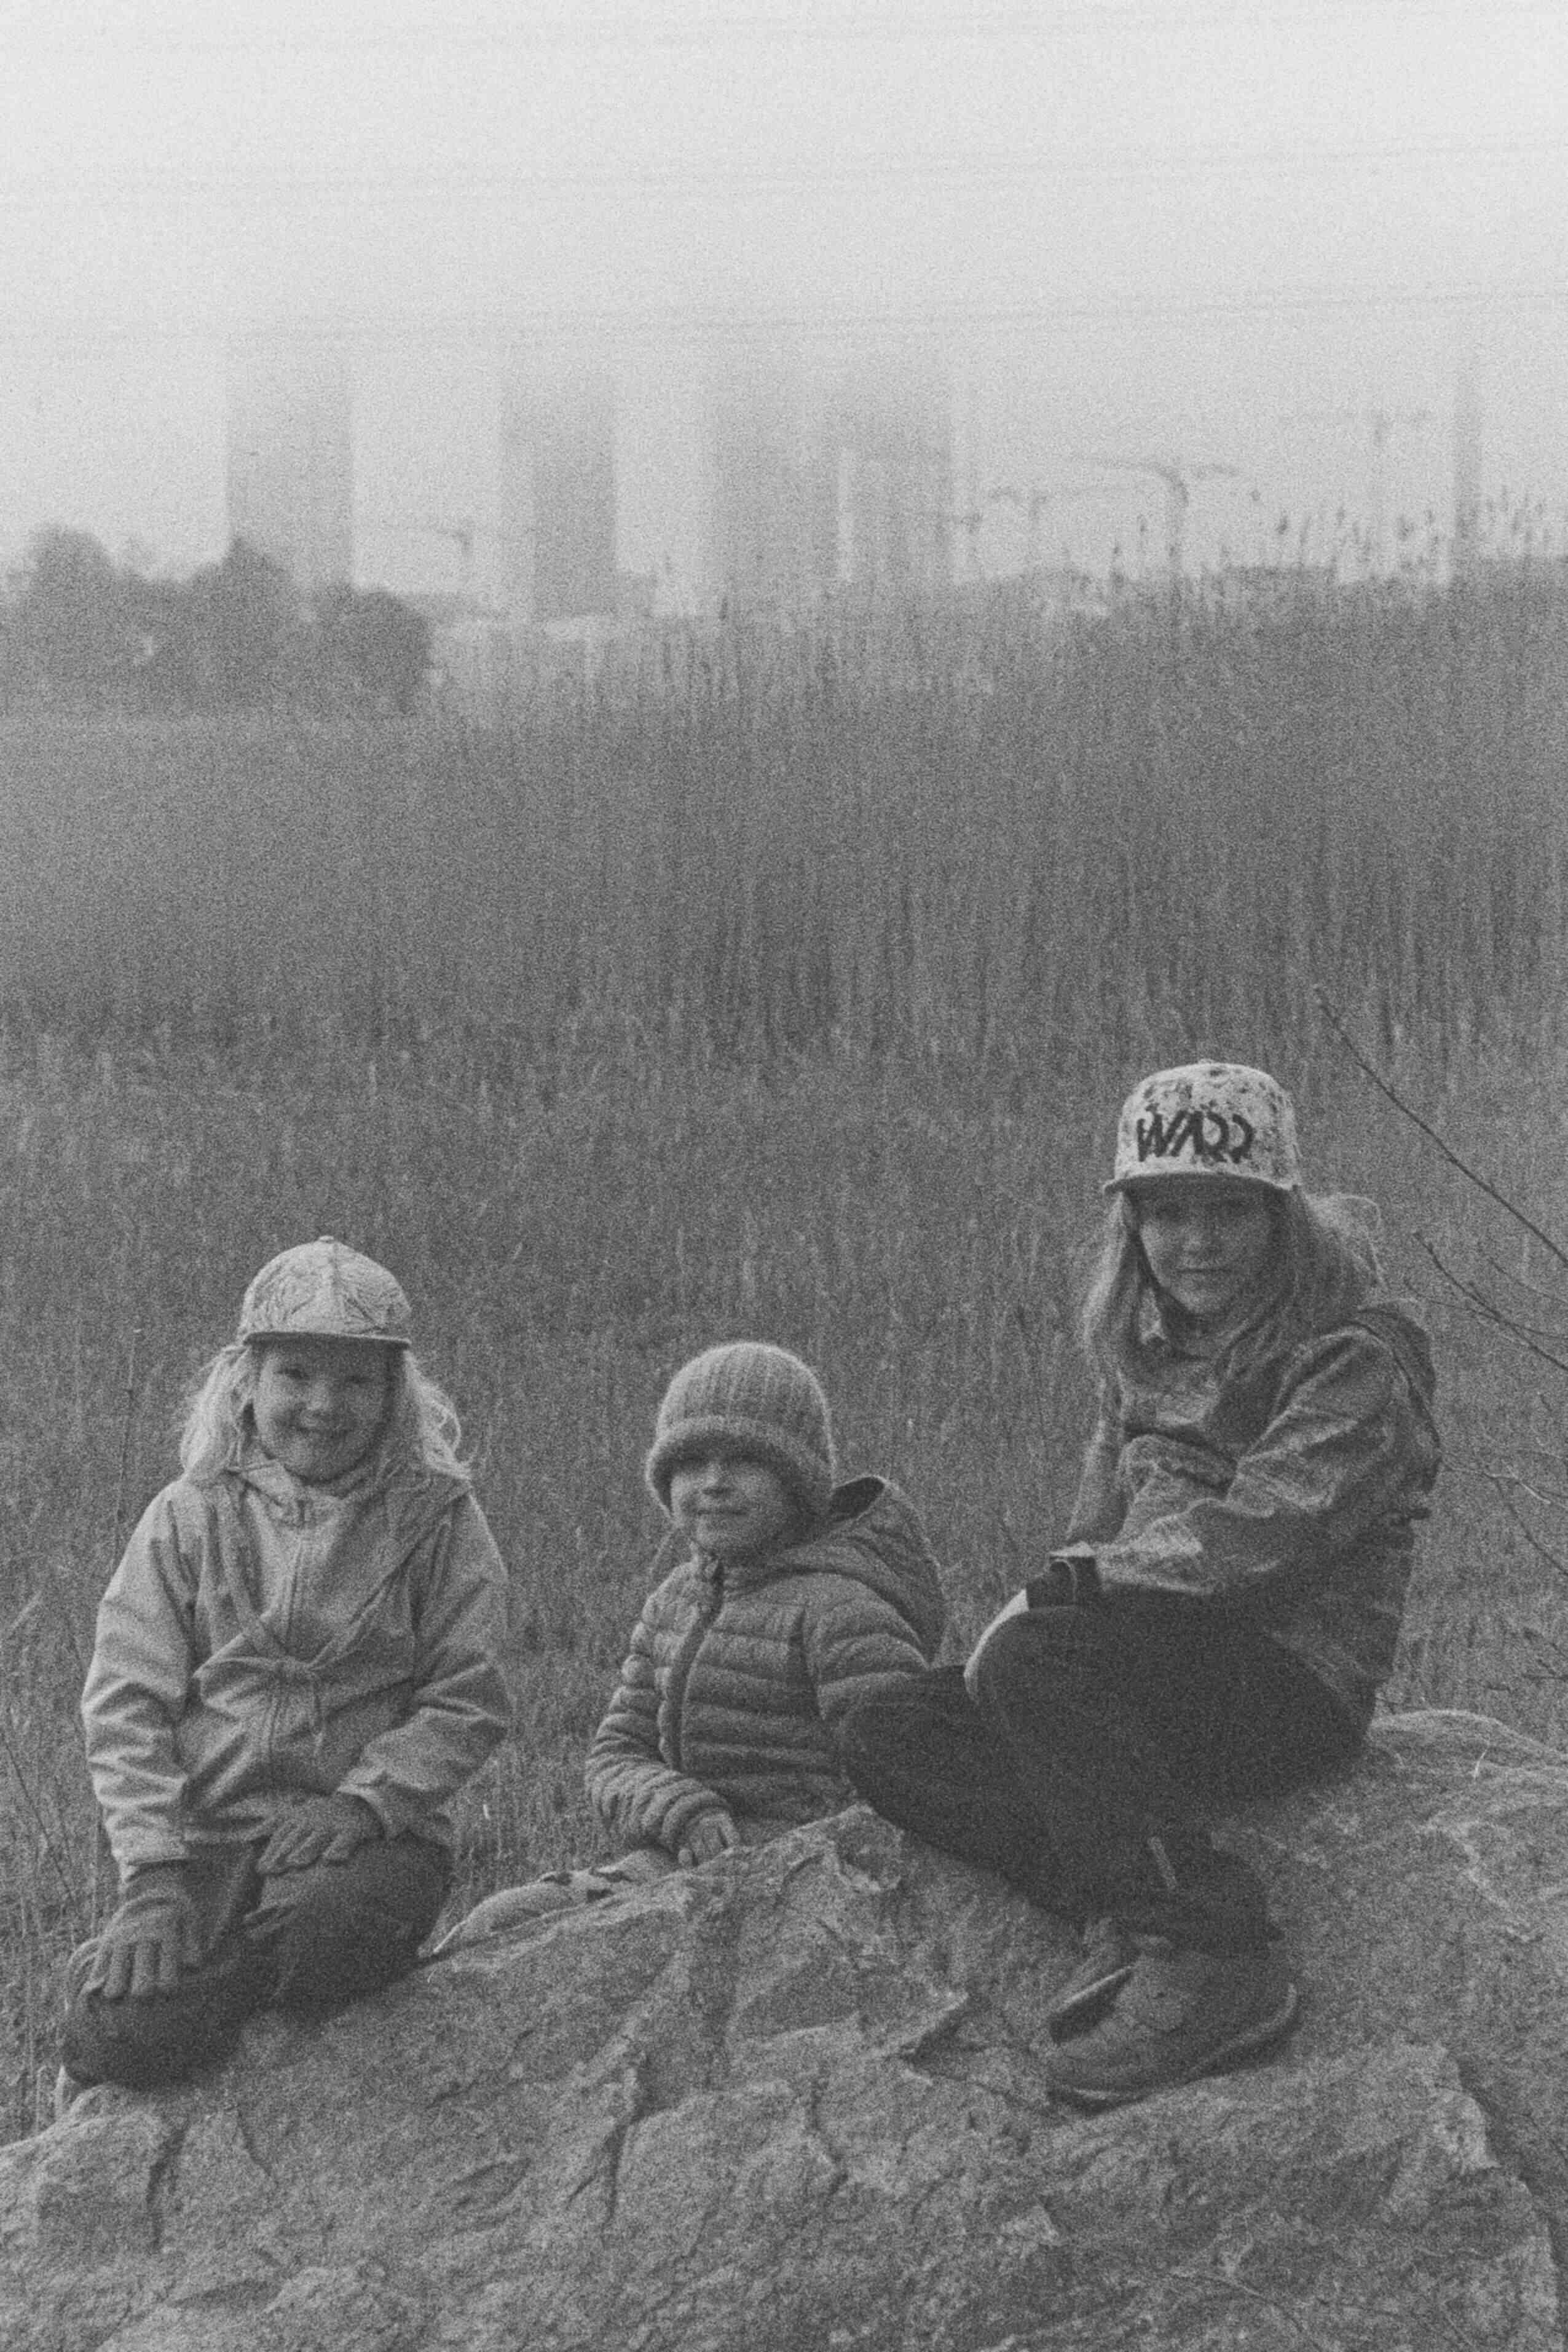
\includegraphics[width=0.8\linewidth]{assets/kolkkienpäiväretkibw13}
	\end{center}

	% \columnbreak

	Aikaa ei enää ollut lähteä kiertämään Viikin muita lintutorneja, vaan
	rastien jälkeen pidettiin lyhyt evästauko ja päätettiin suunnata
	takaisin kohti Viikin tiedepuiston bussipysäkkiä. Osa retkueesta jatkoi
	Nonnan kyydillä hänen kotiinsa Hiekkaharjuun illan johtajahuoltoa
	varten.




\end{multicols}
\vspace*{1.28cm}

\medskip
\noindent\null\hfill Kuvat: Tanguy Gérôme \& Janne Suomalainen\\
\noindent\null\hfill Teksti: Janne Suomalainen

% \vspace*{-0.64cm}

\clearpage

\textbf{Valokuvausrastin tulos:}

\begin{multicols}{2}

	\centering
	\noindent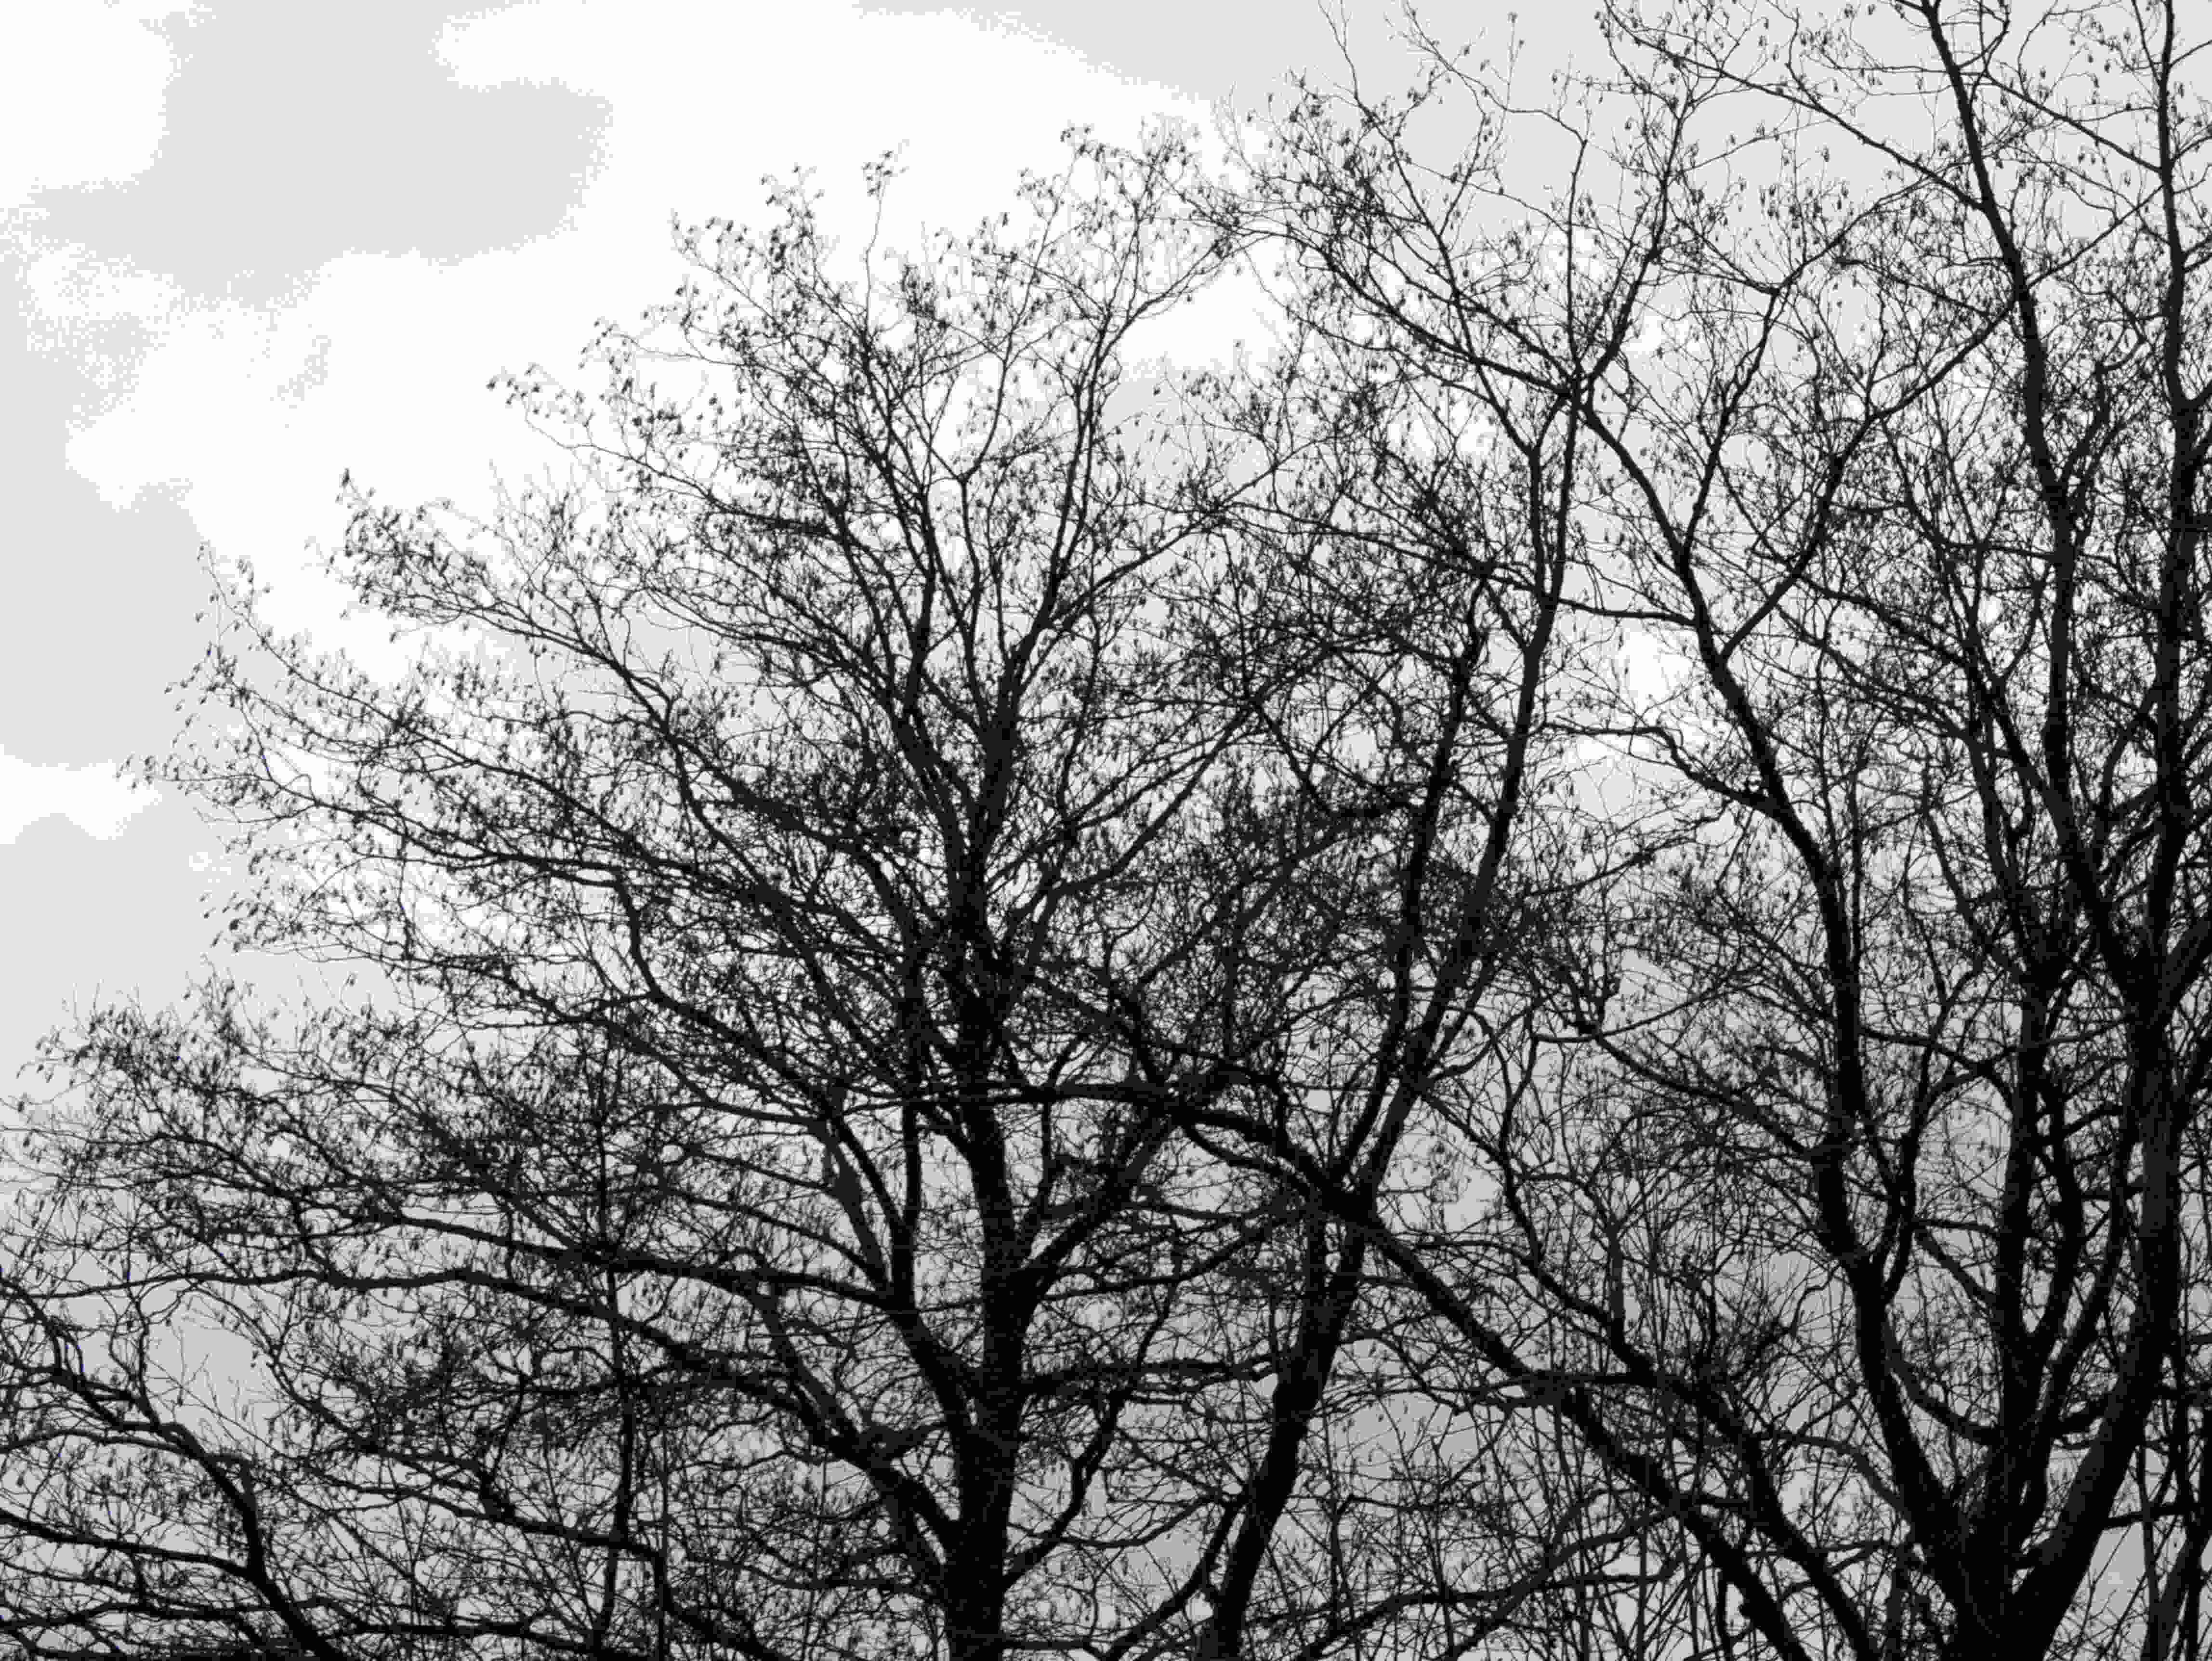
\includegraphics[width=0.9\linewidth]{assets/kolkkienpäiväretki4}
	\noindent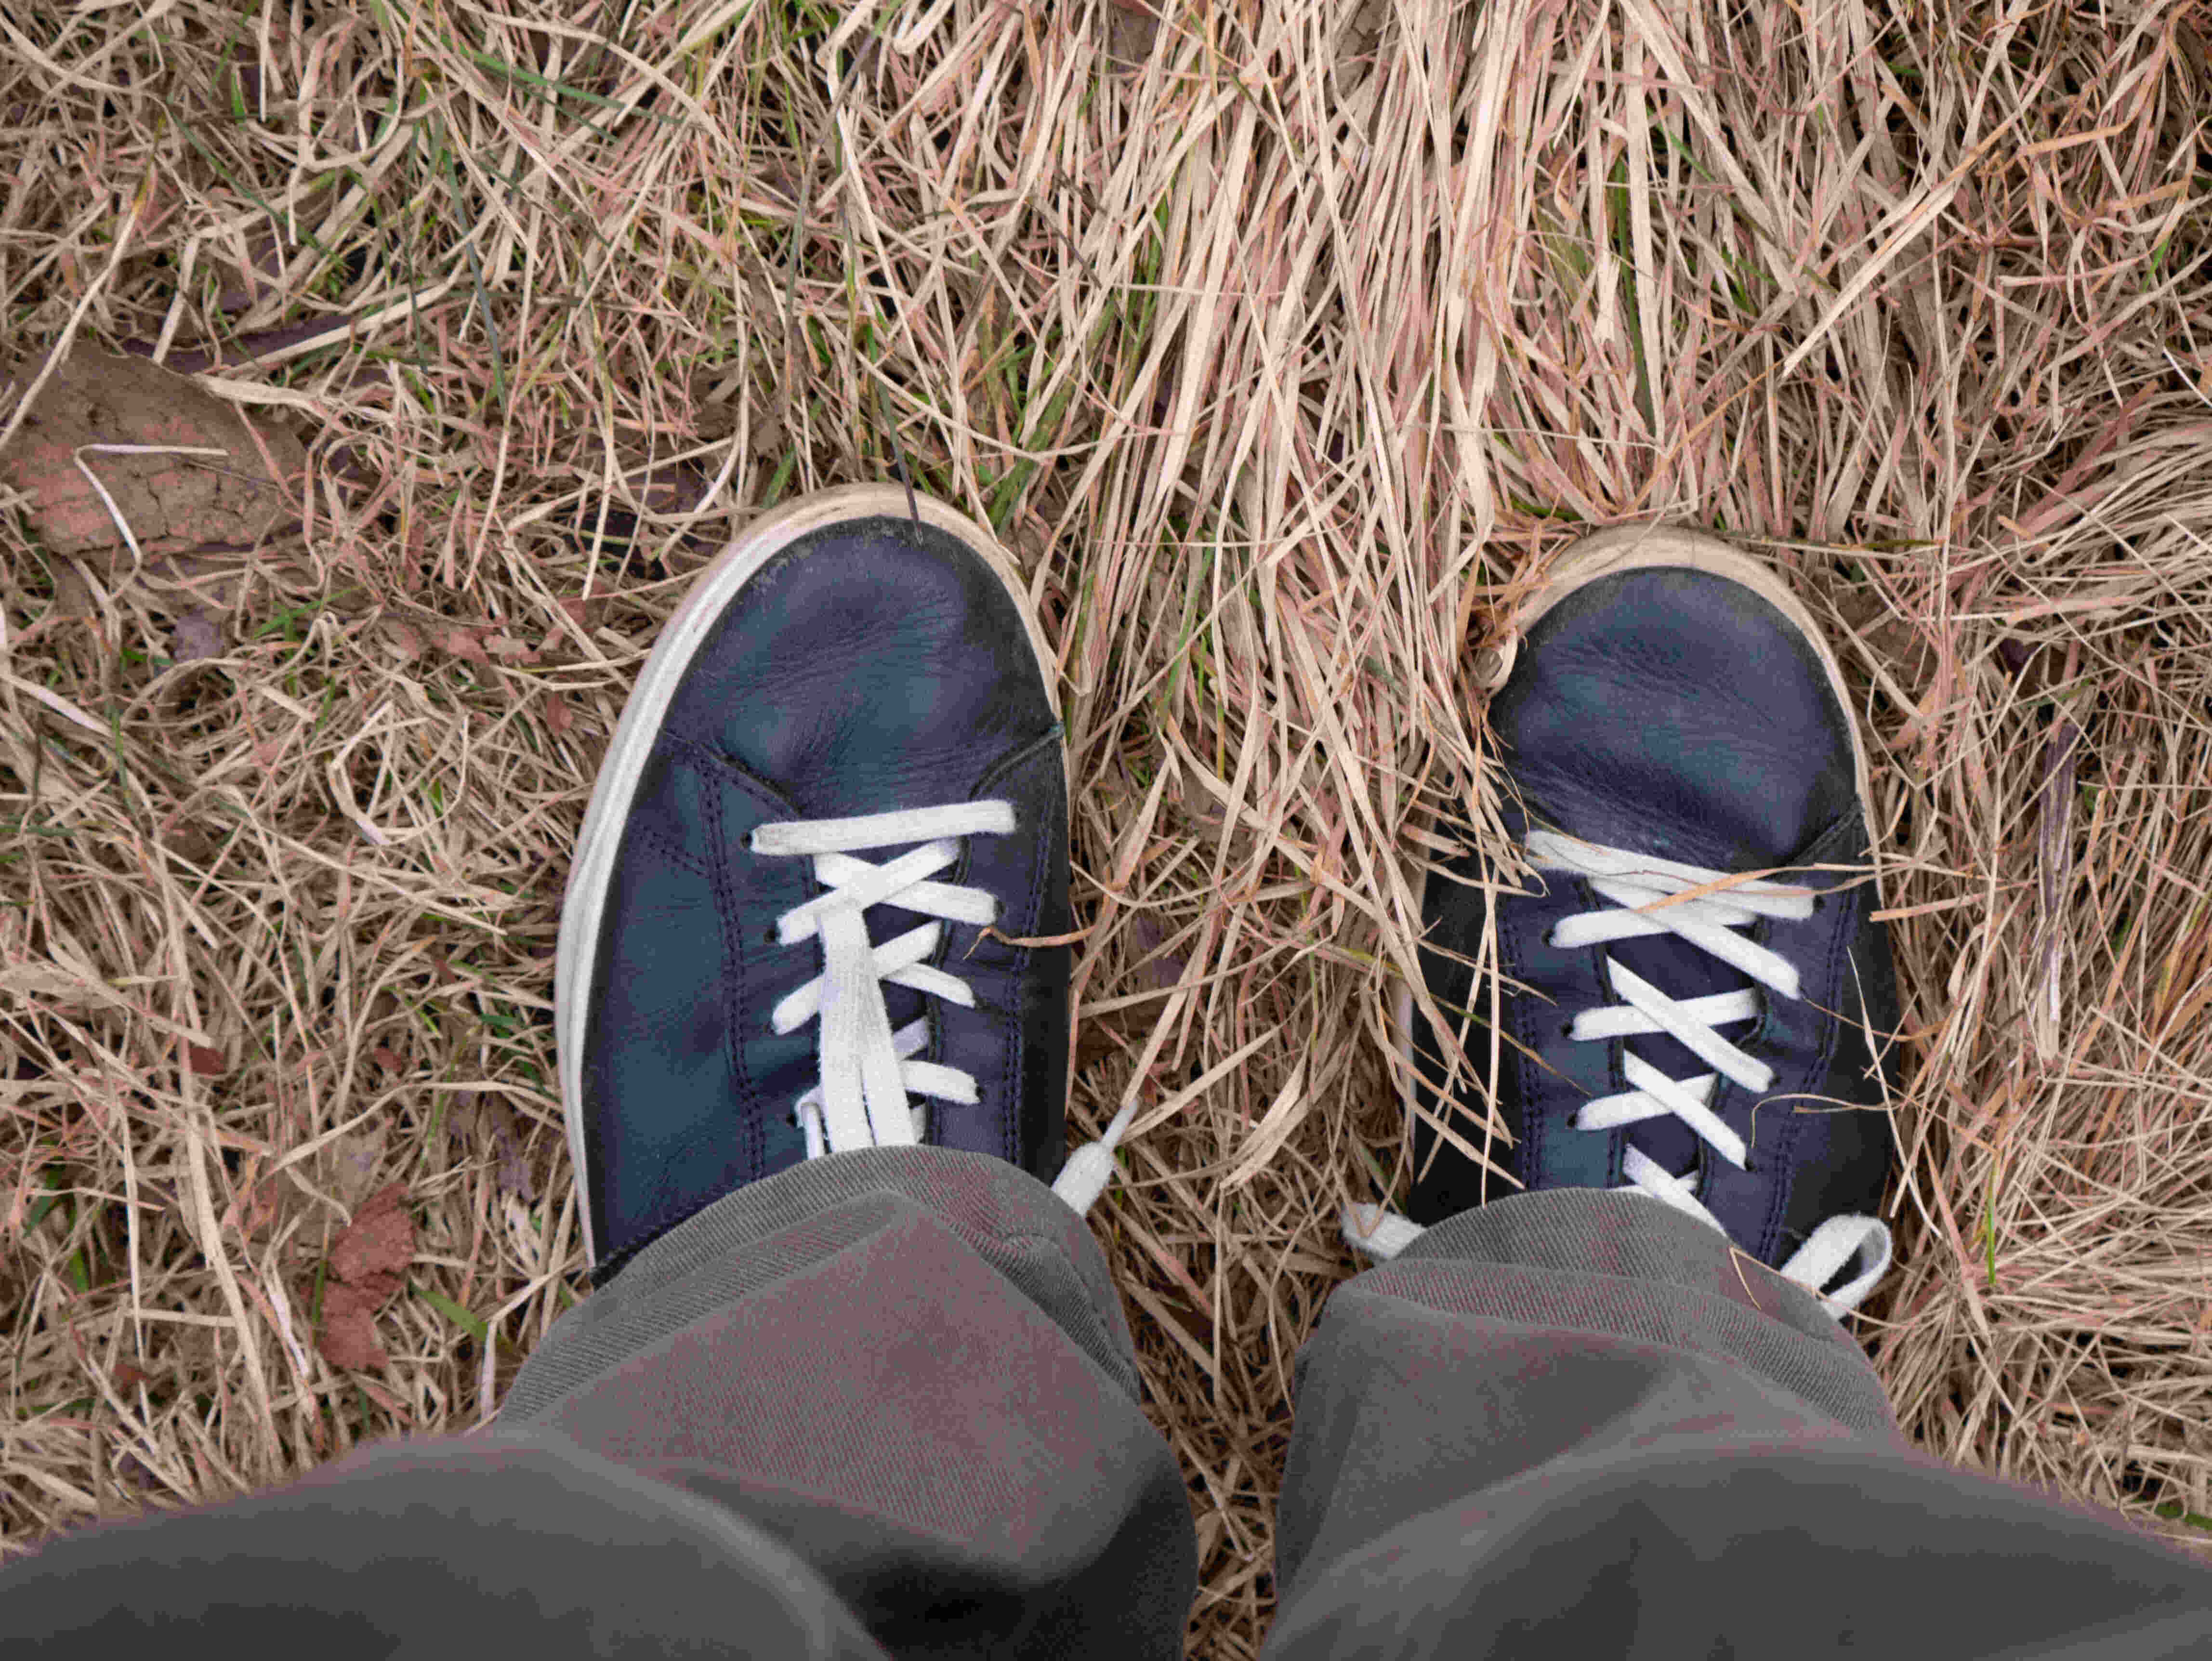
\includegraphics[width=0.9\linewidth]{assets/kolkkienpäiväretki5}
	\noindent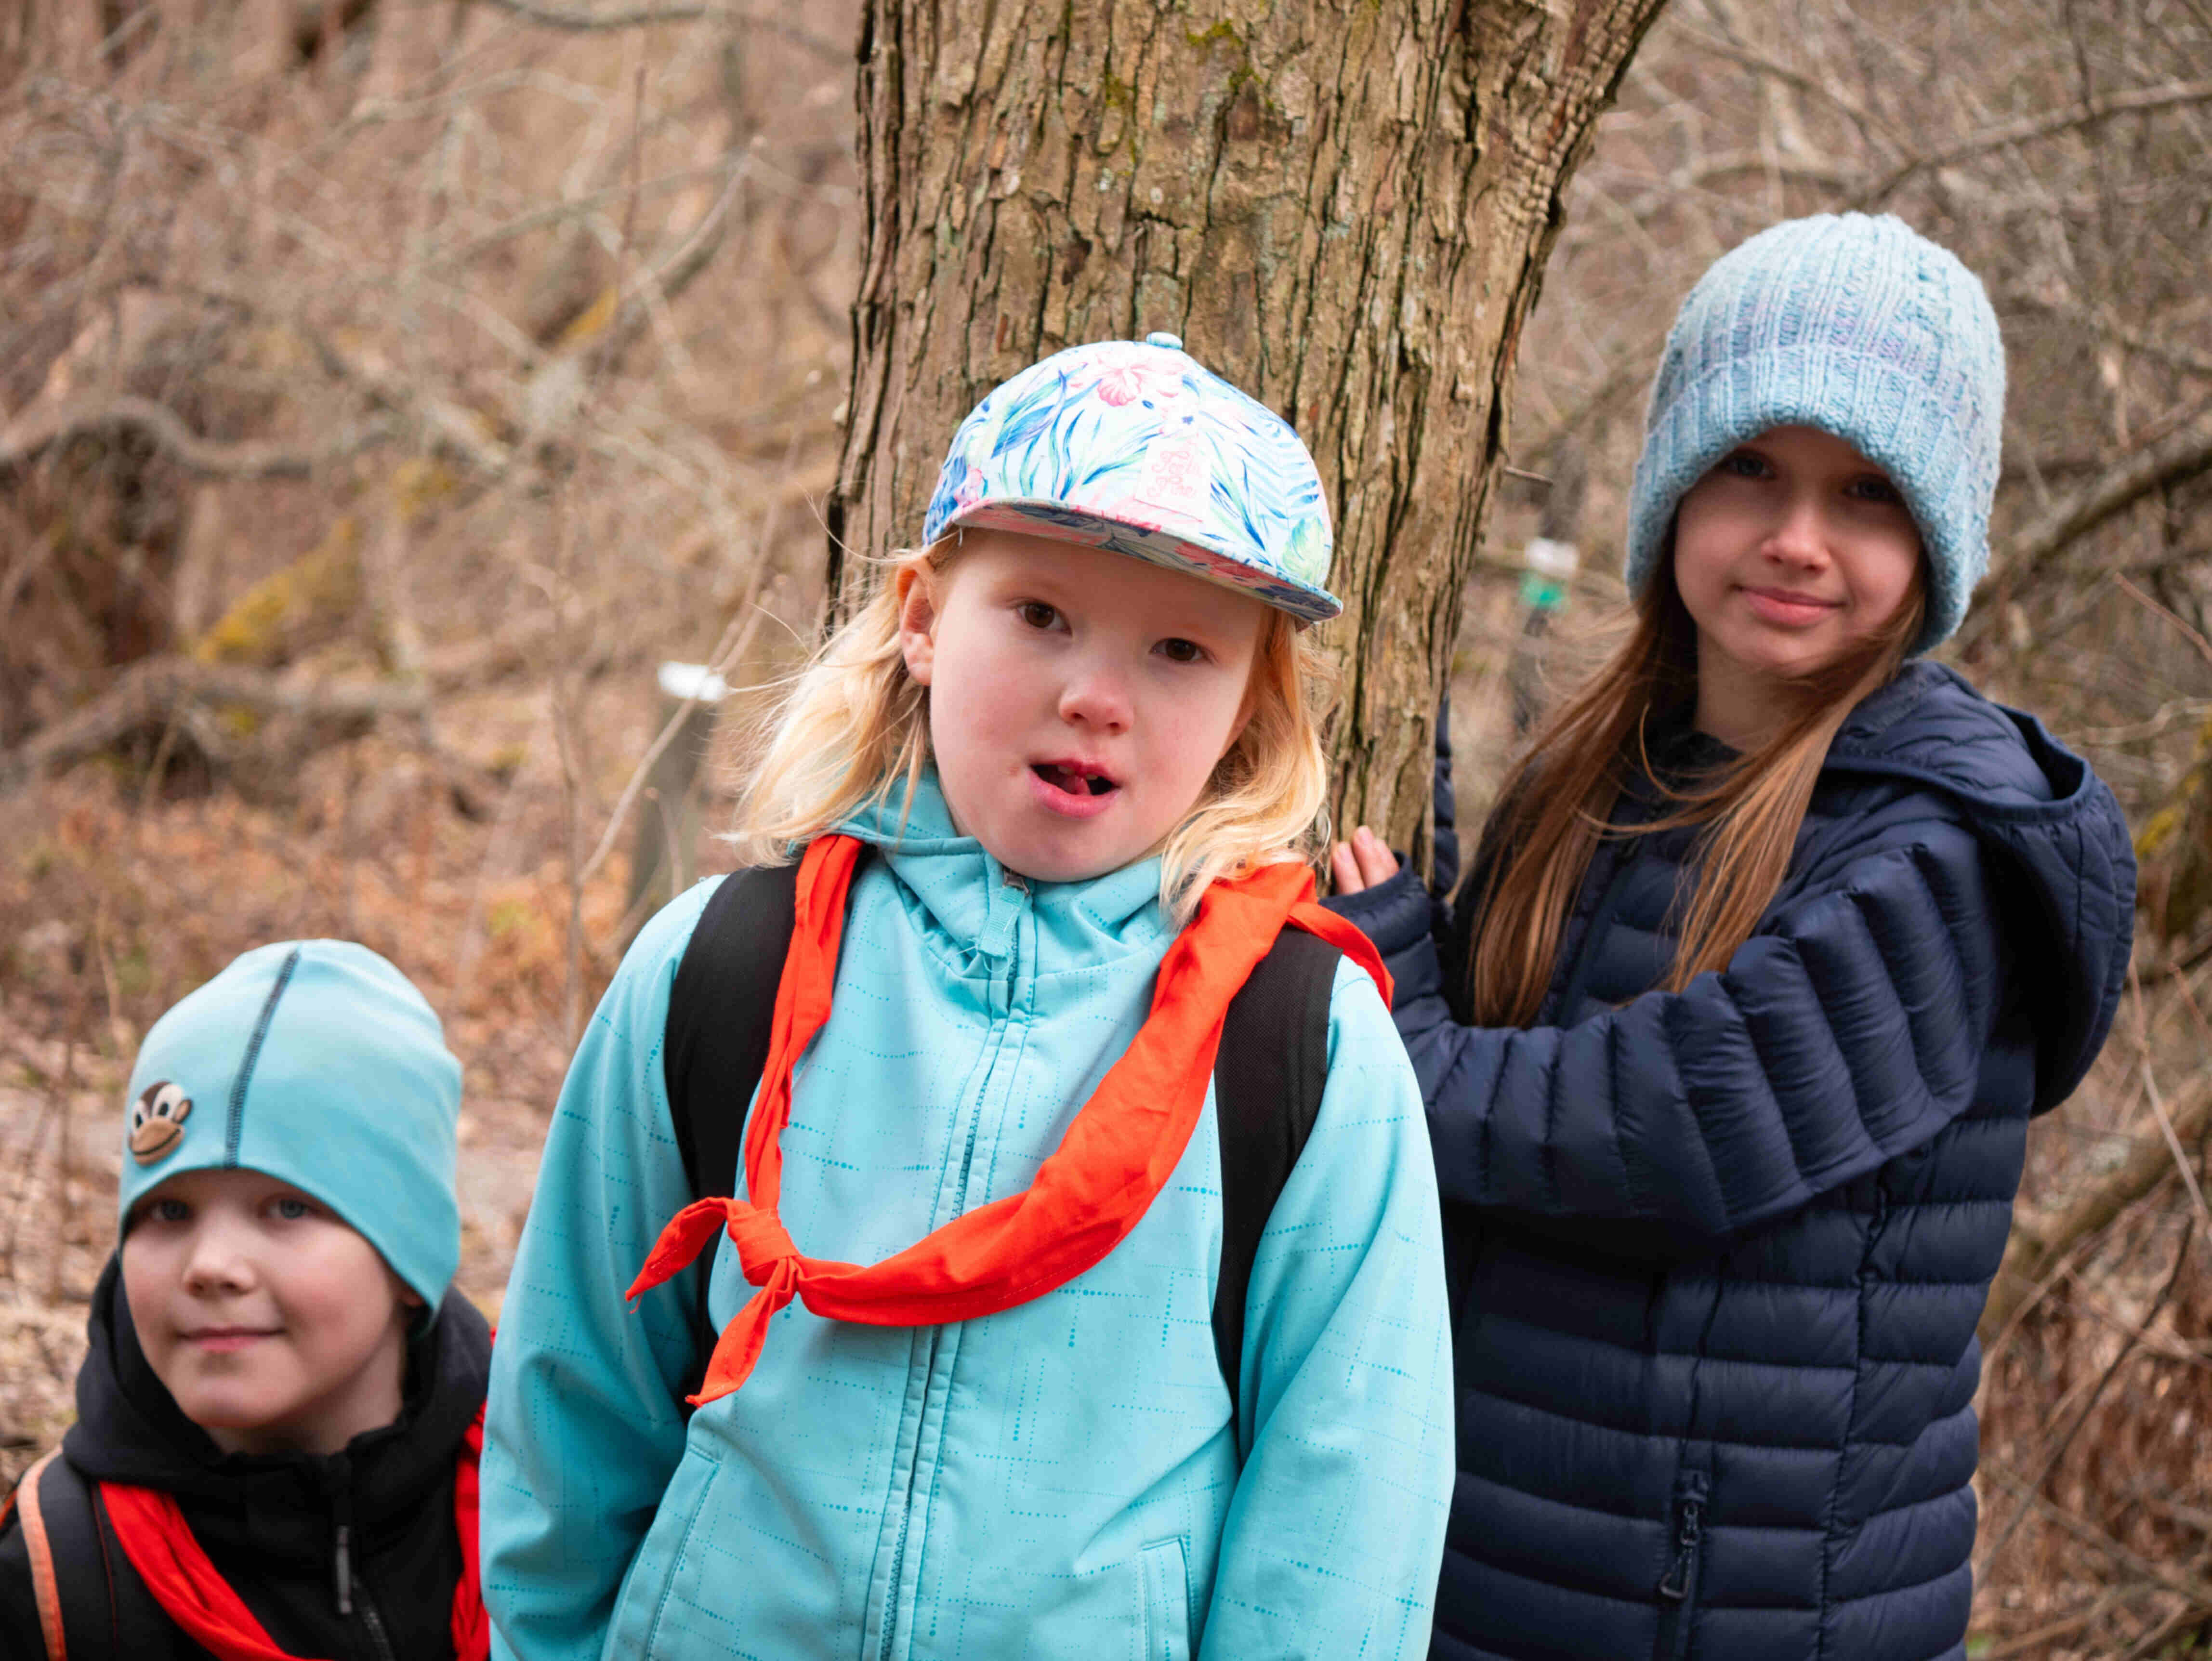
\includegraphics[width=0.9\linewidth]{assets/kolkkienpäiväretki6}
	\noindent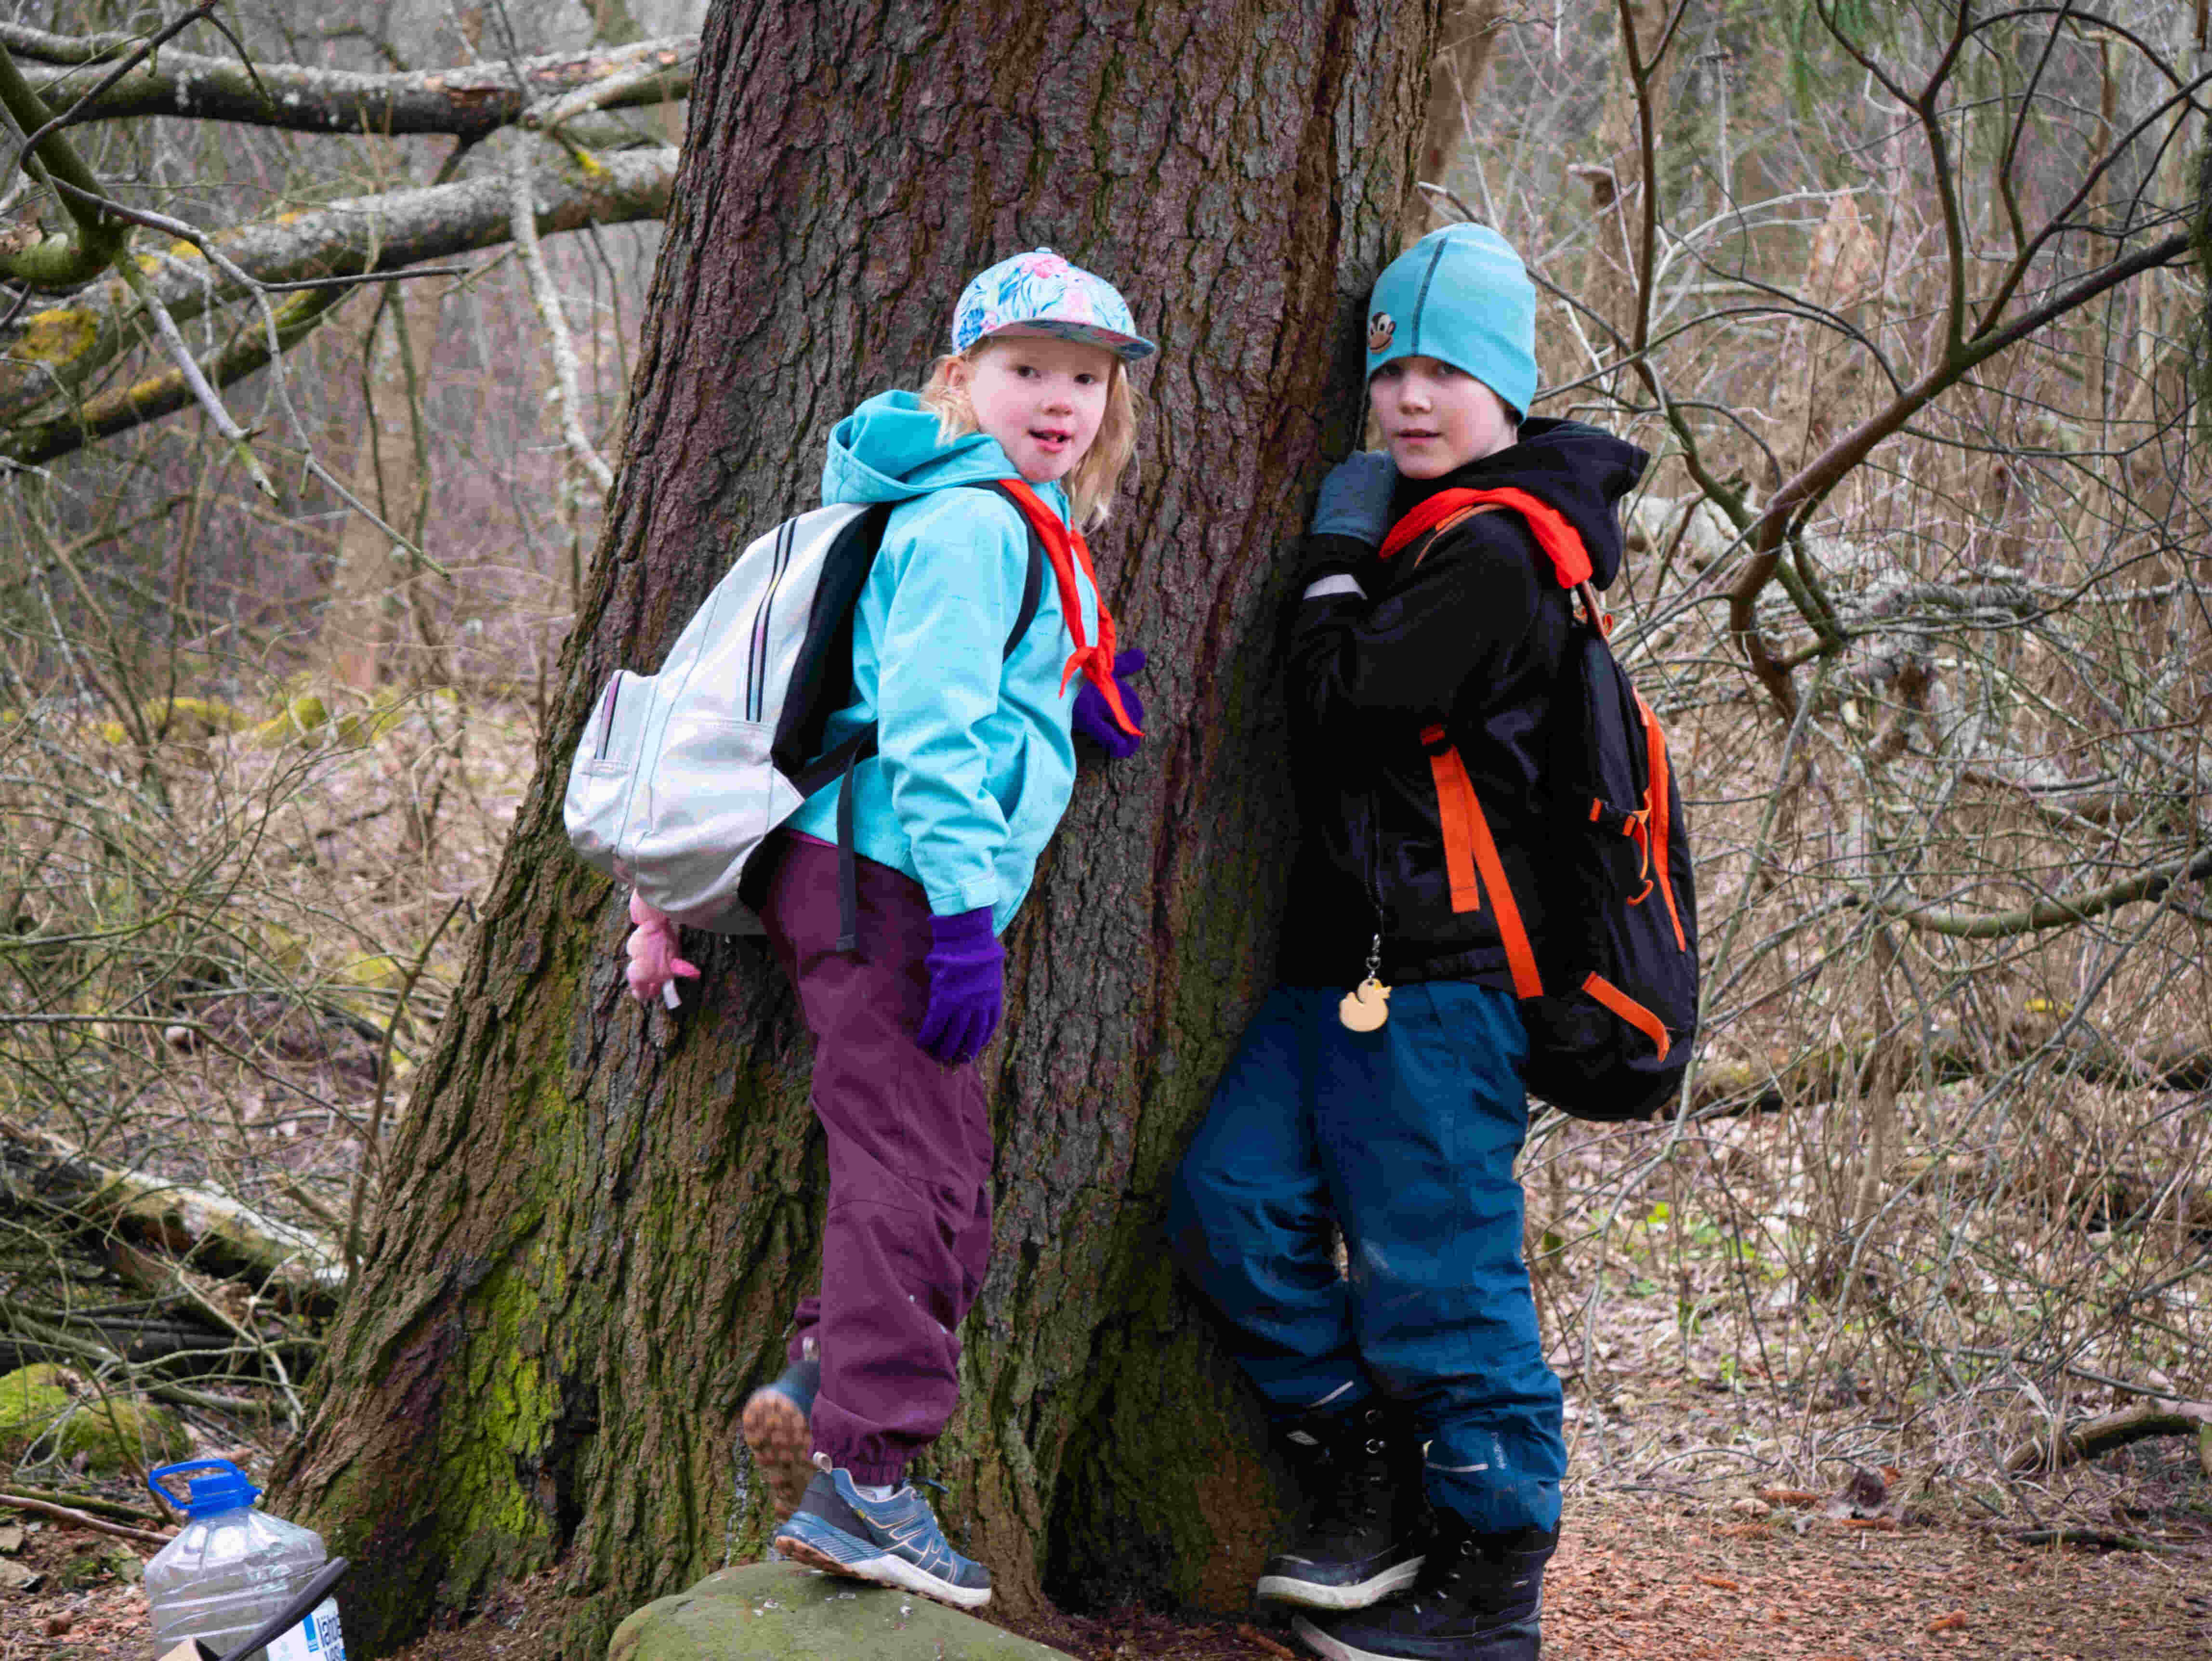
\includegraphics[width=0.9\linewidth]{assets/kolkkienpäiväretki7}
	% \noindent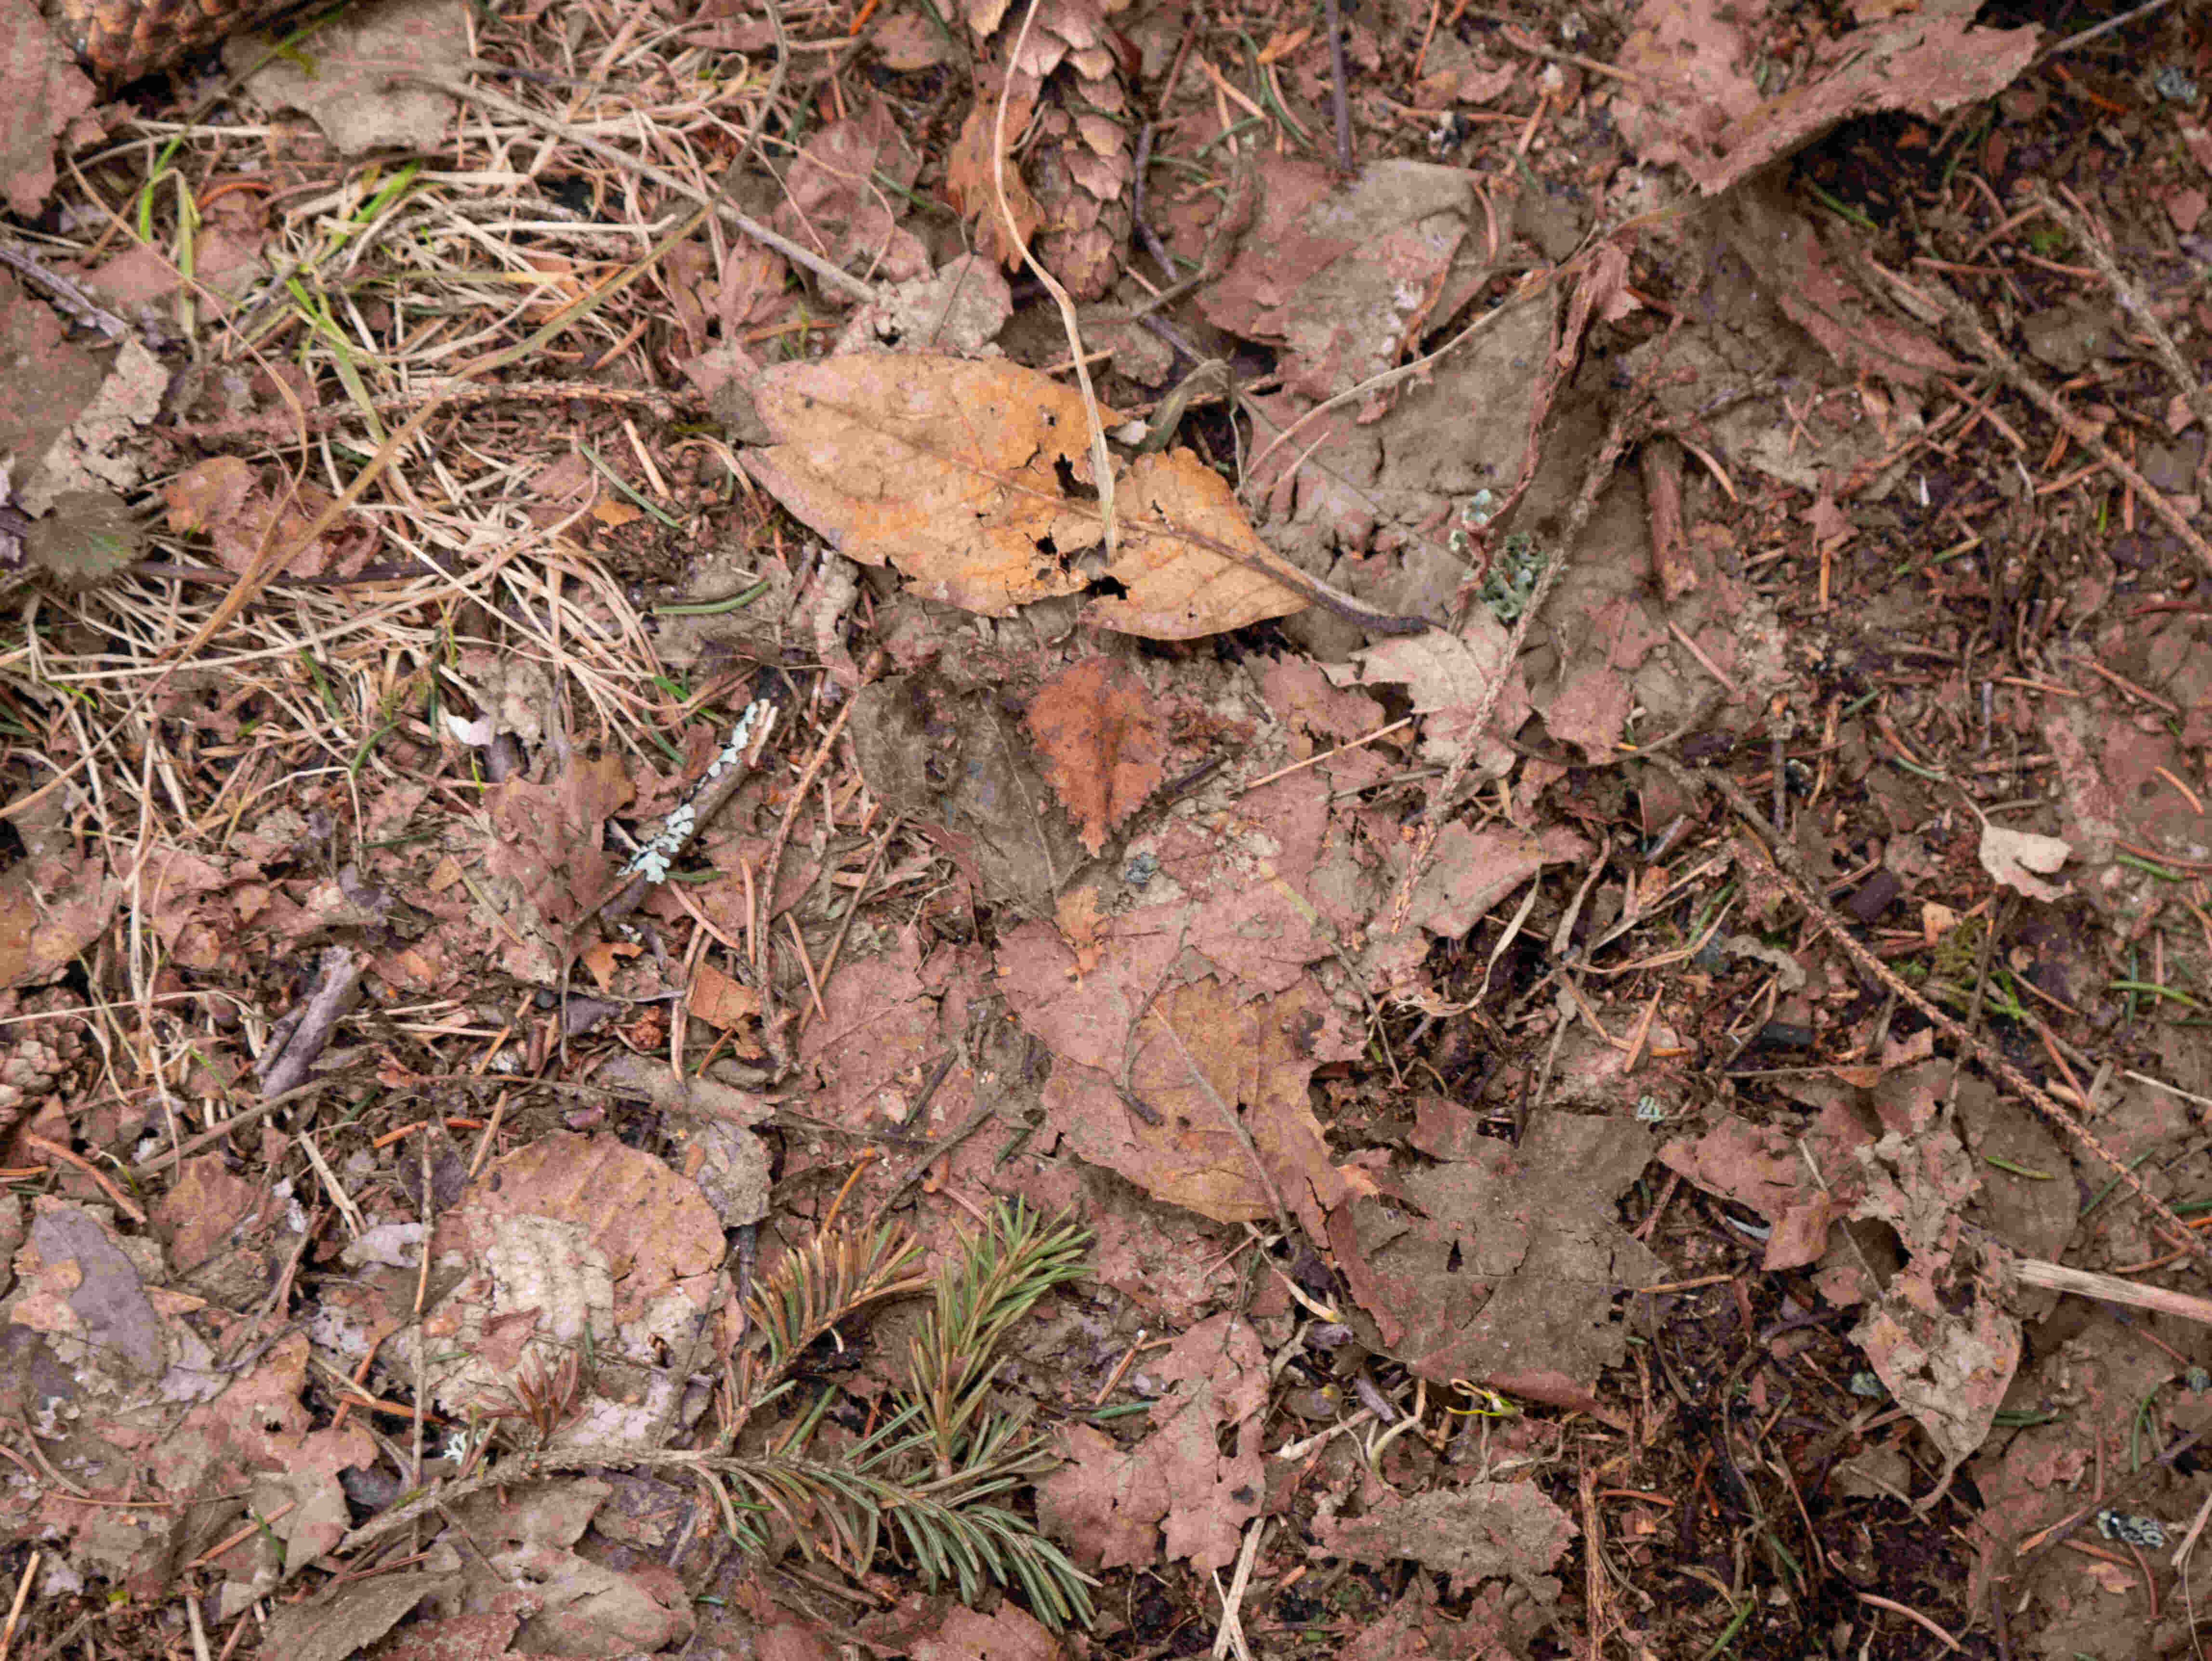
\includegraphics[width=0.9\linewidth]{assets/kolkkienpäiväretki8}
	\noindent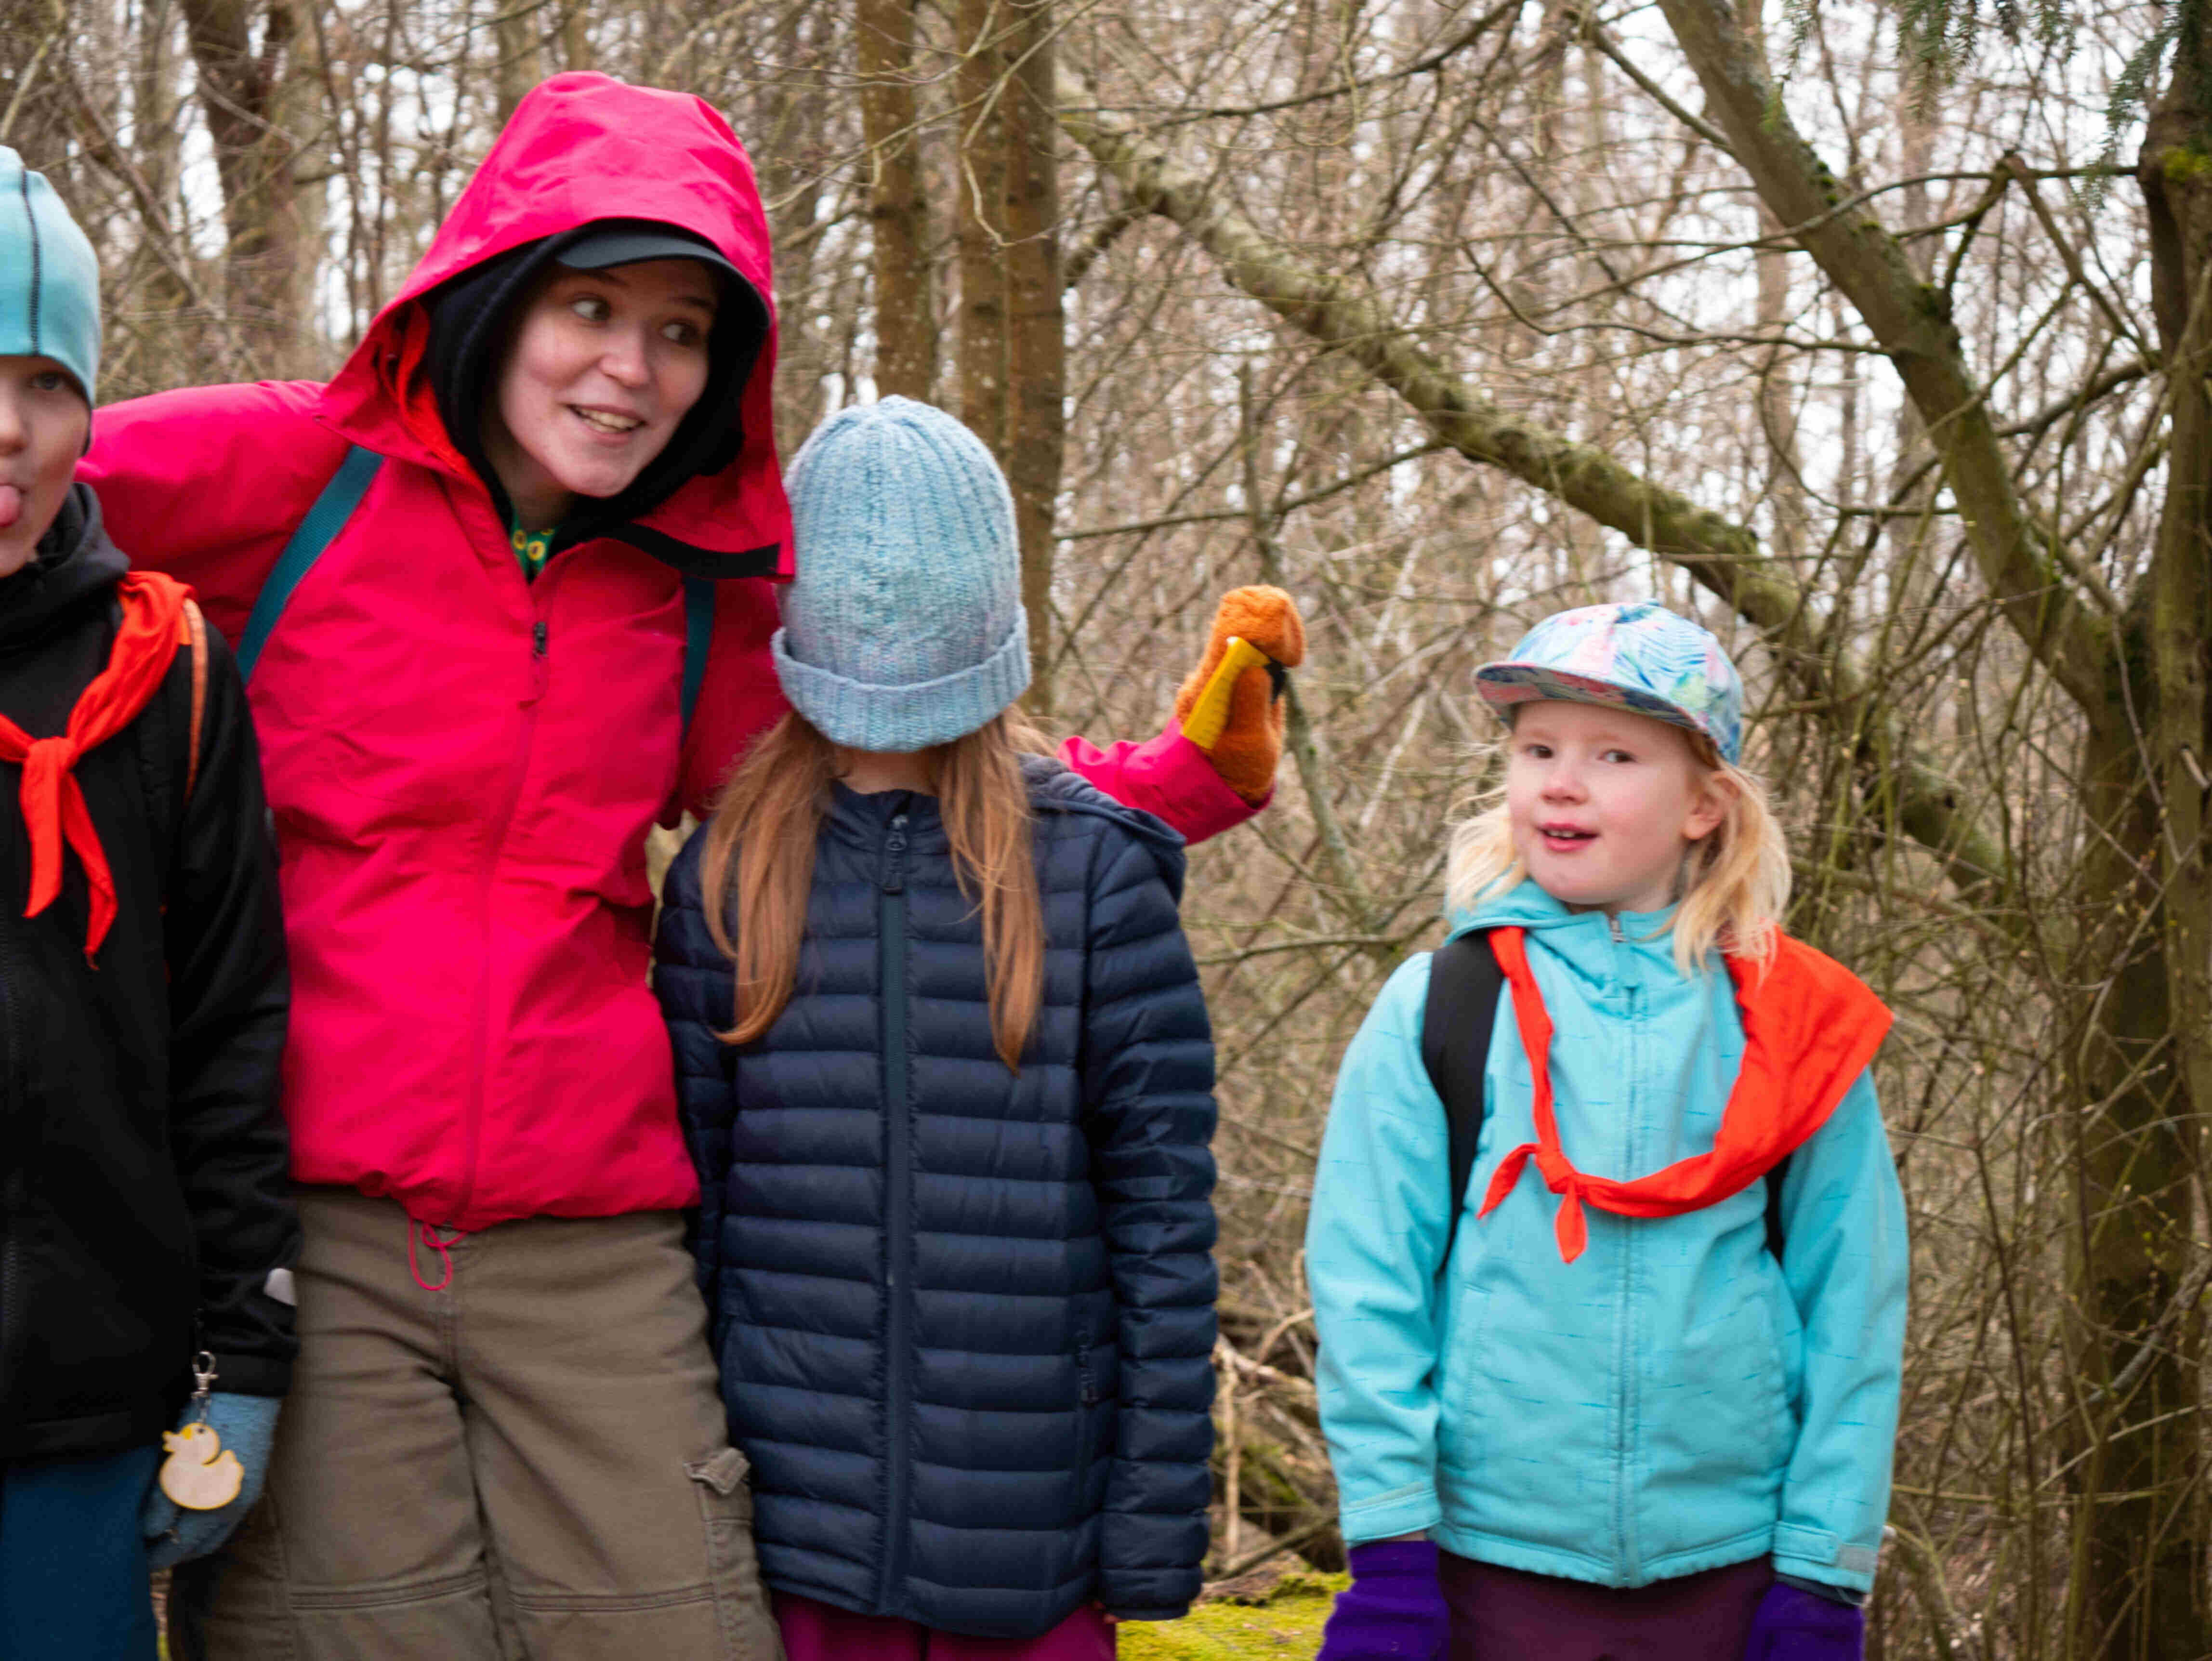
\includegraphics[width=0.9\linewidth]{assets/kolkkienpäiväretki9}
	\noindent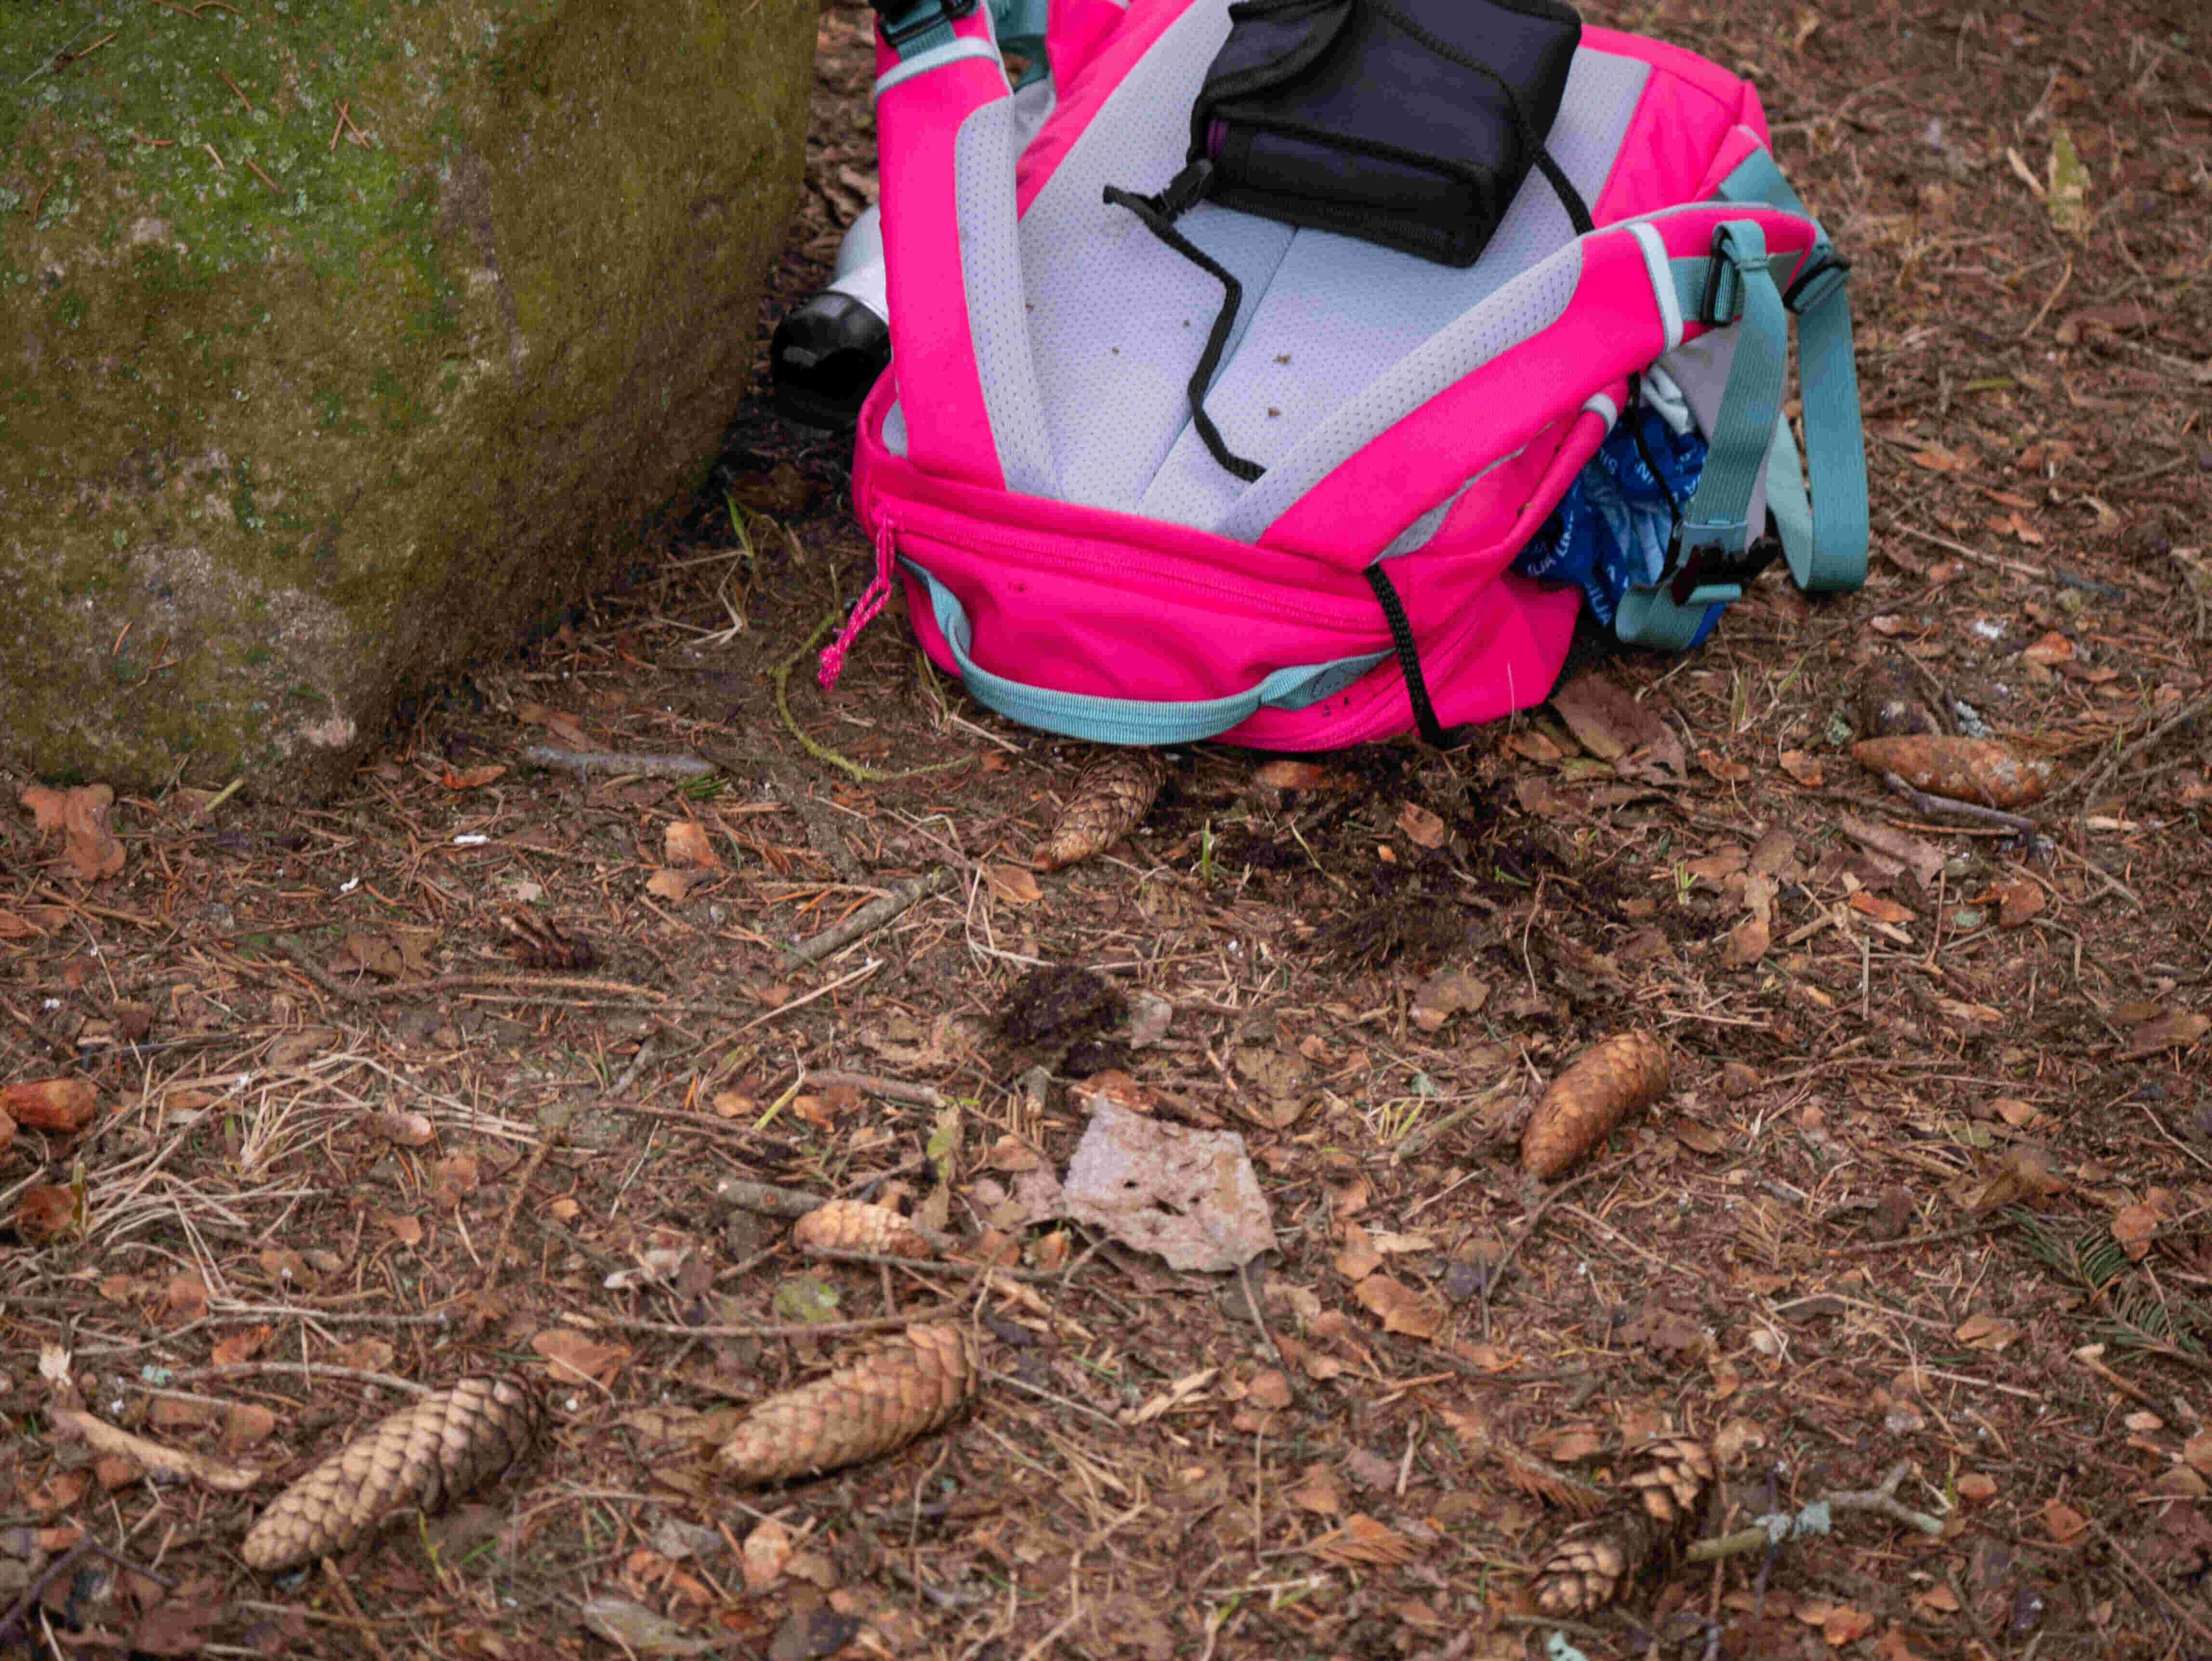
\includegraphics[width=0.9\linewidth]{assets/kolkkienpäiväretki10}
	\noindent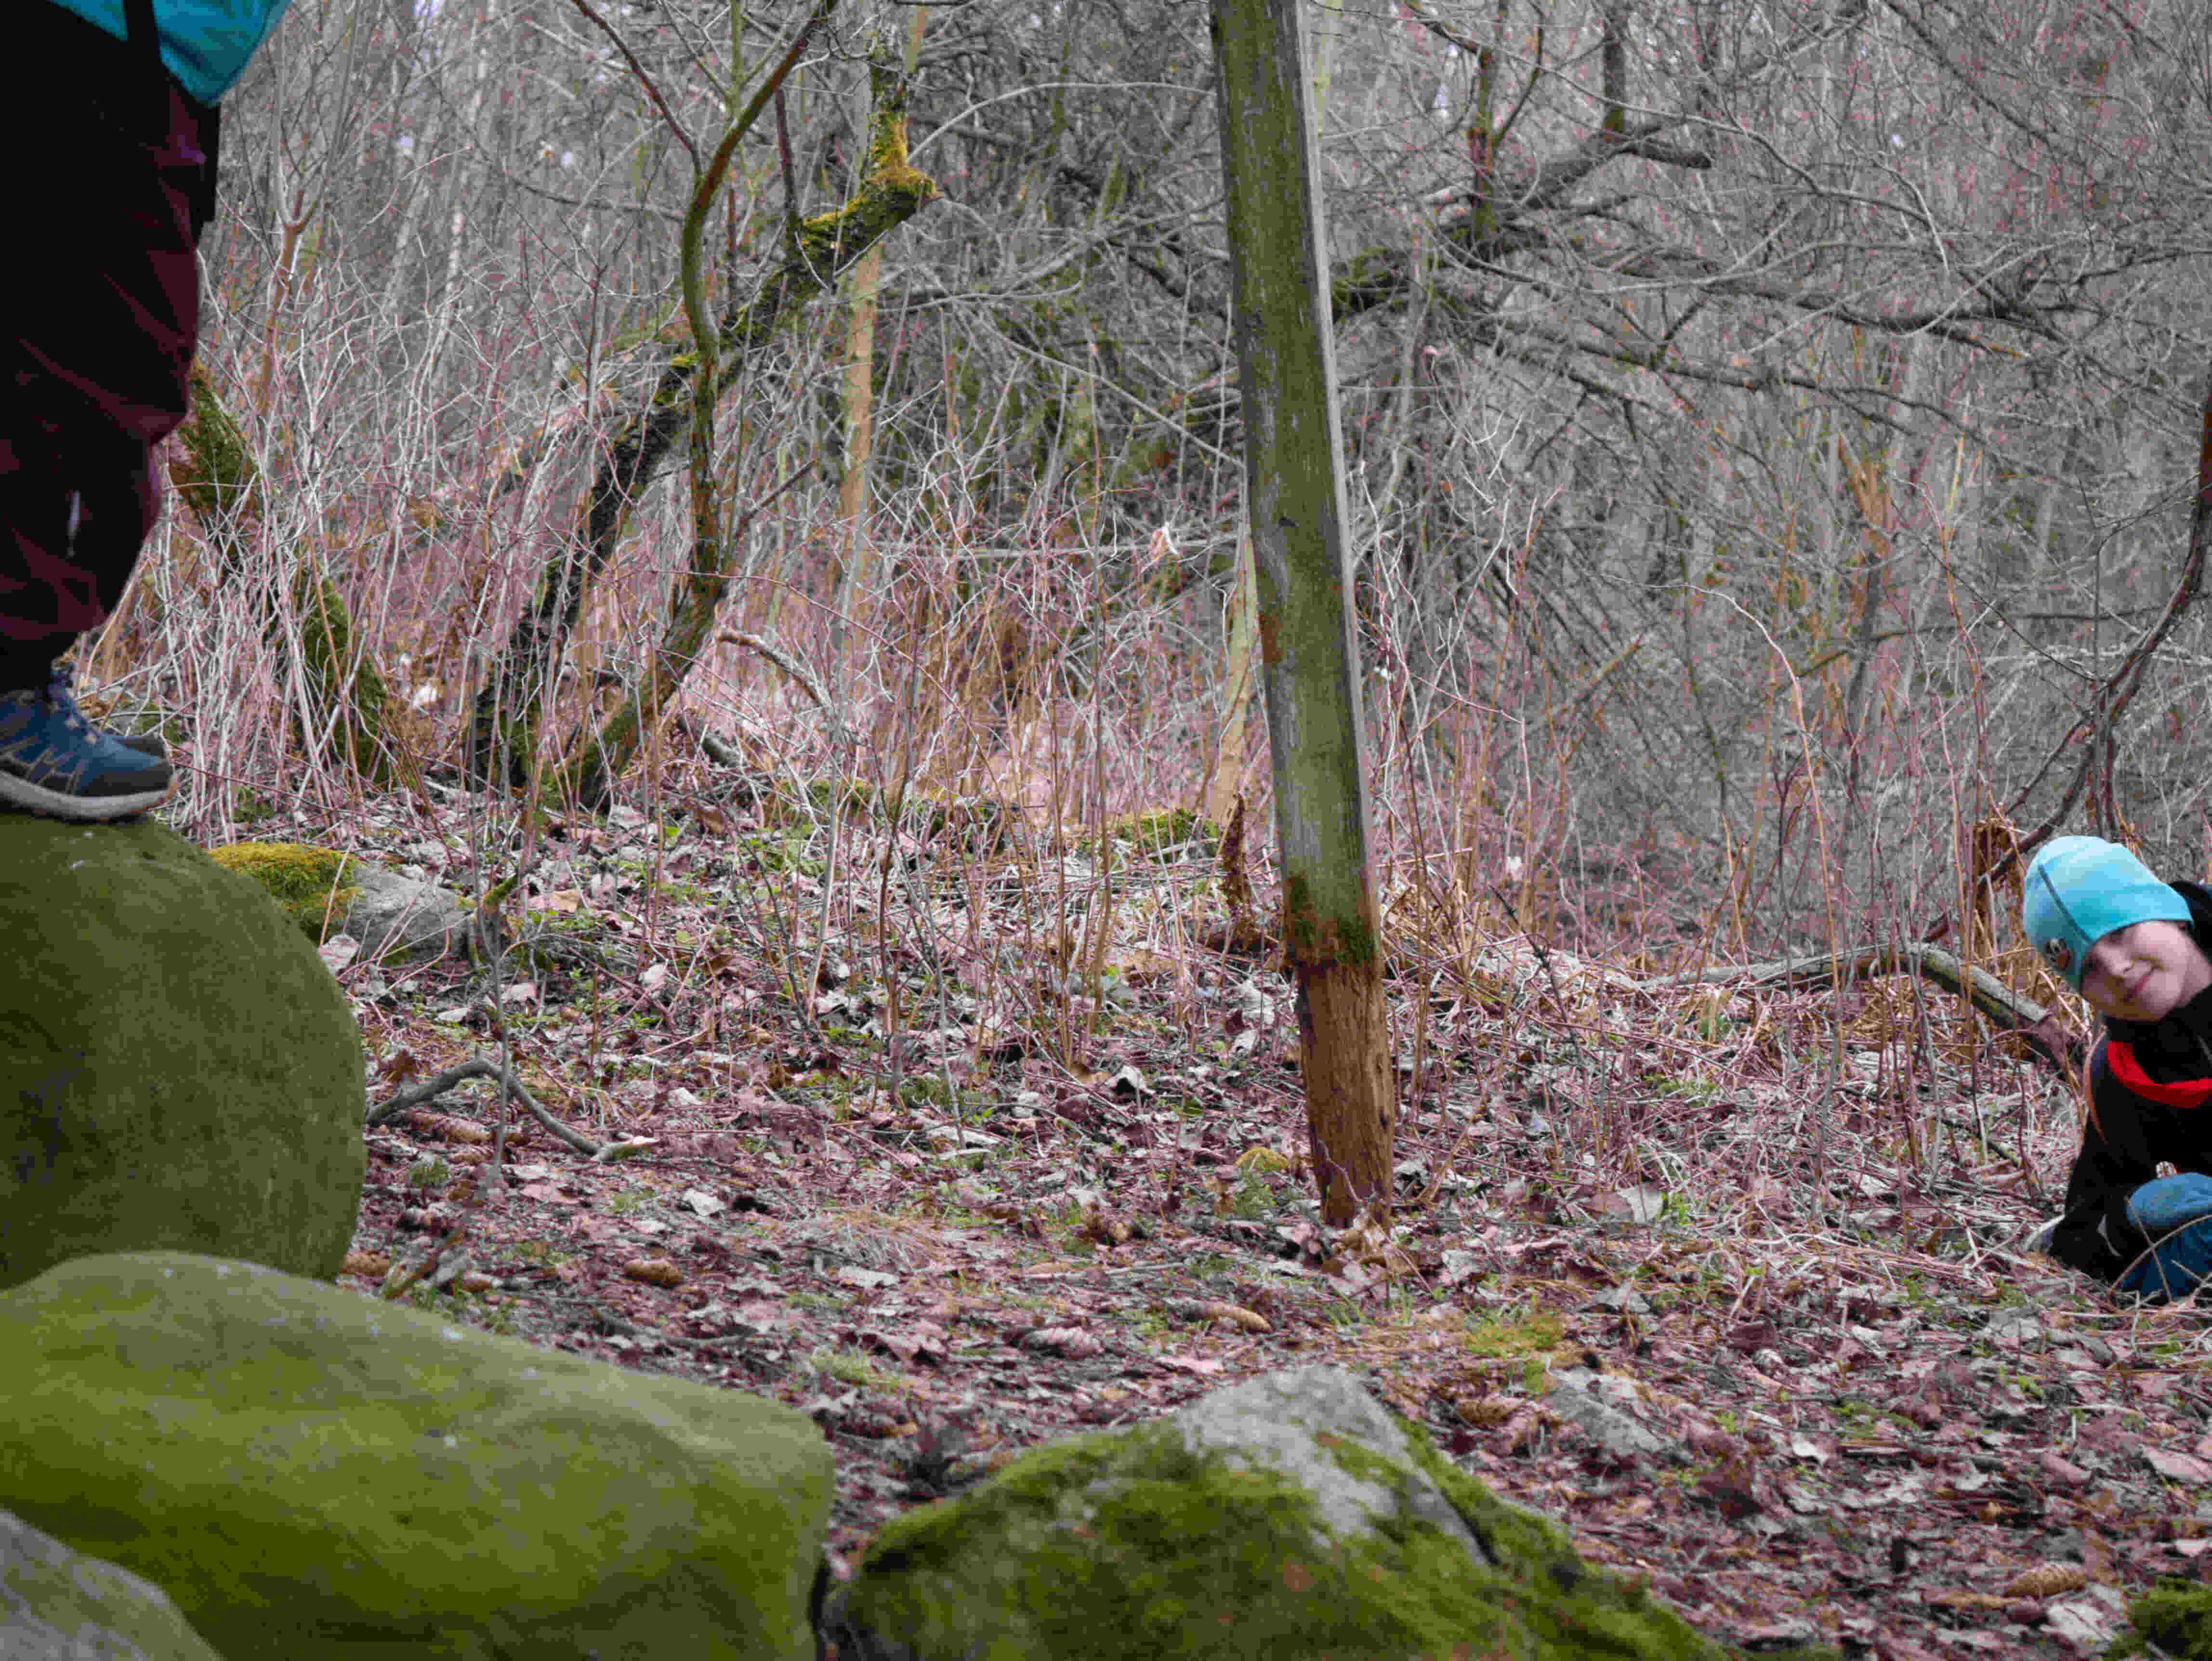
\includegraphics[width=0.9\linewidth]{assets/kolkkienpäiväretki11}
	\noindent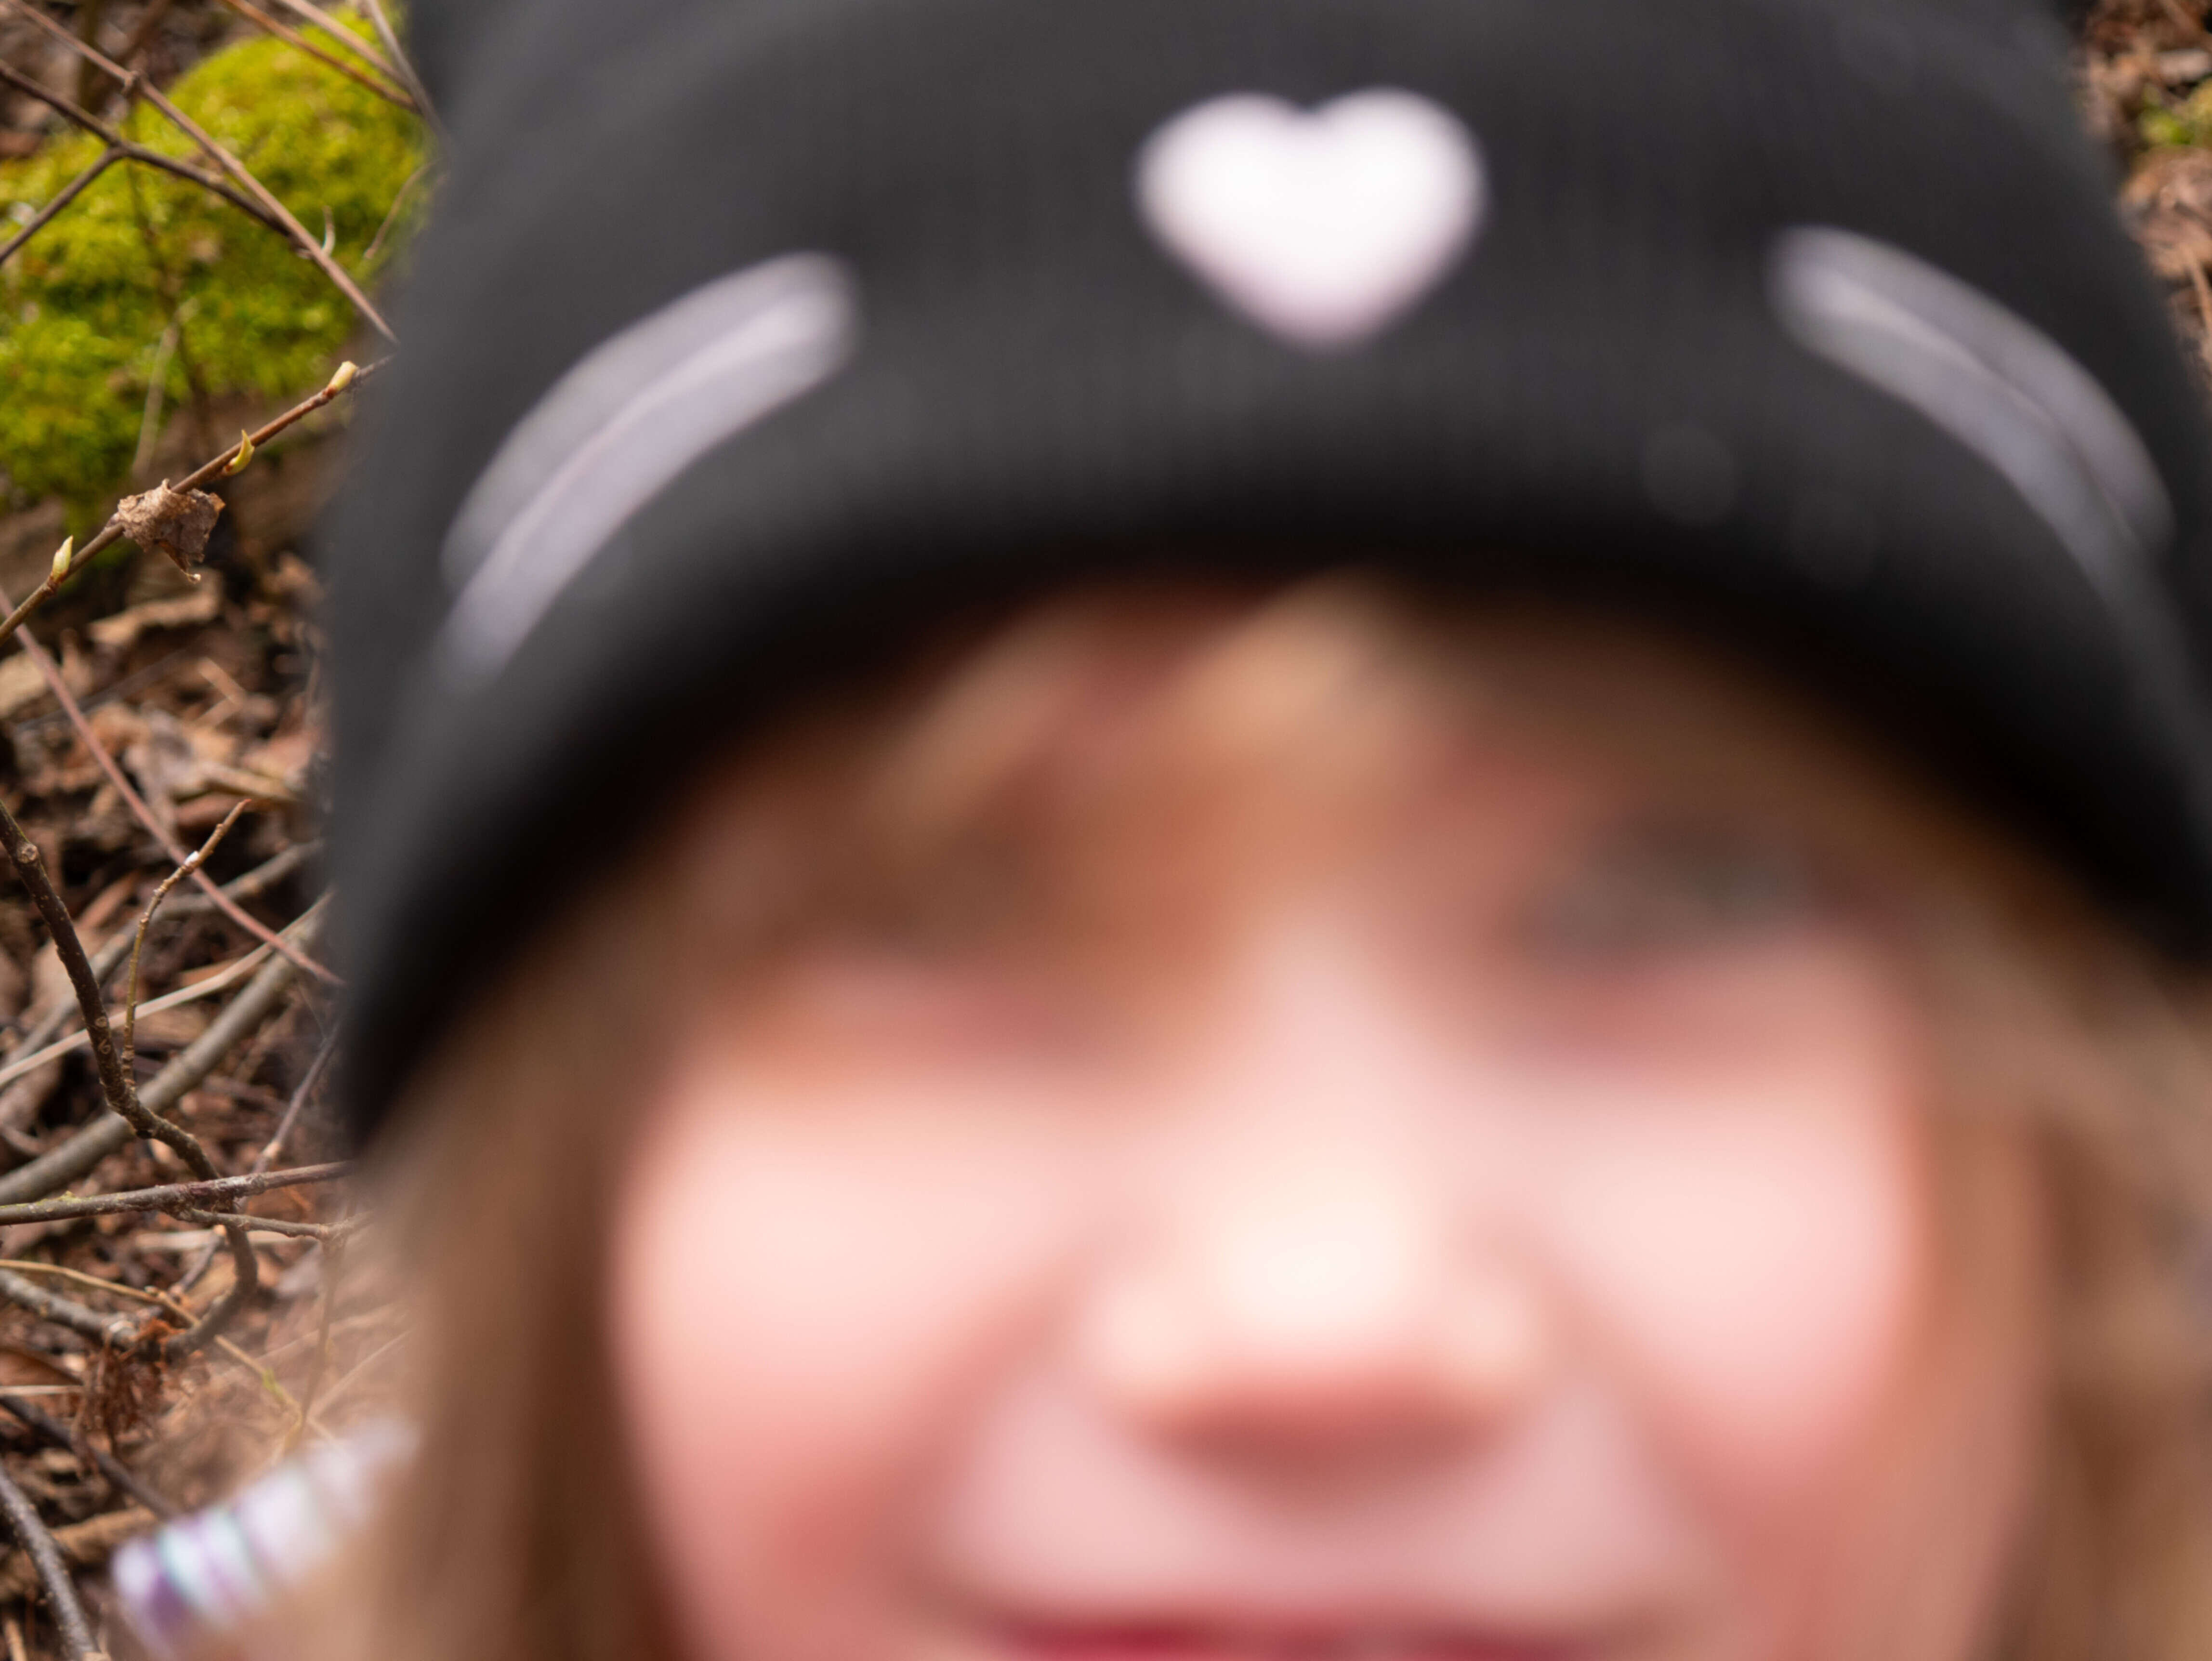
\includegraphics[width=0.9\linewidth]{assets/kolkkienpäiväretki12}

\end{multicols}

